%%%%%%%%%%%%%%%%%%%%%%%%%%%%%%%%%%%%%%%%%%%%%%%%%%%%%%%%%%%%%%%
%
% Beispiel für eine Bachelorarbeit mit FH Aachen
% Titelblattstyles
%
%	Prof. Enning, 18.07.2013
%   Überarbeitet, 17.06.2014
%   Philipp Zähl, 01.02.2019
%   Überarbeitet, 19.08.2021
%
%%%%%%%%%%%%%%%%%%%%%%%%%%%%%%%%%%%%%%%%%%%%%%%%%%%%%%%%%%%%%%%

%%%%%%%%%%%%%% Präambel %%%%%%%%%%%%%%%%%%%%%%%%%%%%%%%%%%%%%%%%
\documentclass [headheight=21pt, footheight=21pt]{scrbook}	% KOMA Klasse für Bücher
%
\usepackage{fhac_styling}	% Style-File für Titelblatt
%
% Einstellen der Optionen für die KOMA Klasse
\KOMAoptions{parskip=true, fontsize=12pt, toc=flat, twoside=true, numbers=nodotatend}
	
% parskip Absätze mit Abstand
% fontsize Standardschriftgröße 
% toc Inhaltsverzeichnis ohne Einzüge
% twoside Zweiseitig setzen
% numbers Nummerierungen nicht mit Punkt abschließen
	
	
%
%%%%%% Immer benötigte Packages
%
\usepackage[T1]{fontenc}		% sonst funktioniert die Silbentrennung bei Umlauten nicht
\usepackage[utf8]{inputenc}	% Eingabedekodierung
\usepackage[ngerman]{babel}	% Silbentrennung und Sprachanpassung
\usepackage{blindtext}		% Blindtext
\usepackage[hidelinks]{hyperref}		% Sprungmarken, z.B. im Inhaltsverzeichnis auf Textpassagen
\usepackage{graphicx}		% Definiert o.a. \includegraphics
\usepackage{textcomp}		% Sonst funktioniert z.B. \texteuro nicht
\usepackage[automark,headsepline=0.75pt]{scrlayer-scrpage}	% Package zum Definieren der Kopf- und Fußzeilen
\usepackage{amsmath,amssymb}		% Muss sein - Mathesymbole
\usepackage{mathrsfs} 	% Weitere Mathematik-Symbole, z.B. Laplace-L

% Float für Bilderpositionierung
\usepackage{float}

% BIB
\usepackage{natbib}
\bibliographystyle{dinat}
\setcitestyle{authoryear}
%\usepackage[backend=biber,style=authoryear,]{biblatex}
%\addbibresource{literatur.bib}

% Anführungszeichen
\usepackage{csquotes}

%%%%% Anpassung an Formatvorlagen des Fachbereichs
%
\usepackage{helvet}		% Serifenlose Schrift ähnlich Arial
\renewcommand{\familydefault}{\sfdefault}	% als Standardschrift serifenlose Schrift verwenden

\usepackage{geometry} 		% Ränder direkt einstellen
\geometry{a4paper, top=20mm, left=30mm, right=20mm, bottom=25mm} % nach Vorgabe
\linespread{1.5} 		% Zeilenabstand nach Vorgabe

\usepackage{chngcntr}		% Ändert Verhalten von Countern
\counterwithout{figure}{section}	% Figure-Nummerierung nicht bei section-Wechsel zurücksetzen
\renewcommand{\thefigure}{\thechapter.\arabic{figure}}	% im Stil 3.2


\AtBeginEnvironment{quote}{\small\itshape}
\AtBeginEnvironment{itemize}{\setlength{\parskip}{7pt}\small}
\AtBeginEnvironment{enumerate}{\setlength{\parskip}{7pt}\small}

%%%% für das Erzeugen von Grafiken mit Zeichenbefehlen
%
\usepackage{tikz}		% Grundpaket
\usetikzlibrary{shapes,arrows}	% einige Symbolpackages
\usepackage{tikz-cd}		% einige Symbolpackages
%
%%%%%% Gegebenenfalls nützliche Zusatzpackages
%
%\usepackage{blindtext}		% Blindtexte zum Ausprobieren von Formatierungen
%\usepackage{color}		% Schriftfarben
\usepackage{colortbl}		% für die Hintergrundfarbe von Tabellen
%\usepackage{gensymb}		% Definiert Formelzeichen, die im math und im text-Modus gleich aussehen
%\usepackage{wrapfig}		% Definiert die wrapfigure-Umgebung (Bild am Rand von Text umflossen)
\usepackage{pdfpages}		% Einbinden von pdf-Seiten
%
\usepackage{booktabs} 		% Schöne Tabellen
%\usepackage{tabu}	 	% Sehr einfach Tabellen gestalten
%\usepackage{array} 		% Erweiterung der Tabellenumgebung, neue Spaltentypen
\usepackage{paralist}		% Weitere Nummeriungsoptionen, z.b. alphabetisch für enumerate/itemize
%\usepackage{verbatim}		% Verbesserte verbatim-Umgebung (z.b. Programm-Listings)
%\usepackage{subfig}		% Unterfigures mit eigenen Bildunterschriften
\usepackage{afterpage}      % Objekte auf die nächste Seite verschieben
\usepackage{pdflscape}      % Blockweises landscape
\usepackage{tabularx}       % Special Tabellen
\usepackage{longtable}      % Mehrseitige Tabellen
\usepackage{shellesc}       % Ermöglicht shell Befehle
\usepackage{datatool}       % Stapelverarbeitung von Dateien
\usepackage{catchfile}      % Datei auslesen
\usepackage{setspace}       % Zeilenabstand
\newcommand\loaddata[1]{\CatchFileDef\loadeddata{#1}{}}

\usepackage[font={small,it}]{caption}   % Figure Caption individualisieren
\usepackage{subcaption}                 % Kleine Bilder nebeneinander

\usepackage{vcell}       % Spezielle Zellen in Tabellen
\usepackage{multicol}   % Mehrere Spalten für Listen
\usepackage{enumitem}   % Custom enumerate Label

\newcommand{\imagewidth}{0.85\textwidth}
\def\checkmark{\tikz\fill[scale=0.4](0,.35) -- (.25,0) -- (1,.7) -- (.25,.15) -- cycle;} % Häkchen


% Autoren in Kapitälchen
\makeatletter
\def\NAT@nmfmt#1{\textsc{#1}}
\makeatother
% ----


 % Abkürzungsverzeichnis
 
%\usepackage{glossaries}
%\makeglossaries
%\input{glossar}
 
%%%%%% Sammelsurium
%
%\renewcommand{\labelitemii}{$\circ$} % Bullets für itemize-Listen
%

%%%%%%%%%%  Angaben für Titelseite %%%%%%%%%%%%%%%%%%%%%%
% Angaben für Titelseite
\arbeitstyp{Mathematische Algorithmen - Ausarbeitung}
\fachbereich{Electrical Engineering and Information Technology}
\studiengang{Information Systems Engineering}
\vertiefung{}
\titel{Kostenminimale Flüsse}
\subtitel{}
\autor{Anton Kamps, Leo Müller, Steffen Richter \& Philipp Zähl}
\matrnr{}
\betreuer{Prof. Dr. rer. nat. Dr.-Ing. Georg Hoever}
\cobetreuer{}
\extbetreuer{}
\datum{\today}
\dank{}

%%%%%%%%%%%%%%%%%%%%%%%%%%%%%%%%%%%%%%%%%%%%%%%%%%%%%%%%%%%


\begin{document}

% Einige Anpassungen müssen nach \begin{document} stehen !!
%\renewcaptionname{ngerman}{\figurename}{\textbf Bild} 	% Bild ... statt Abbildung ... 
\renewcaptionname{ngerman}{\contentsname}{Inhalt}% Inhalt statt Inhaltsverzeichnis


%%%%%%%%%%%%%%%%%%%%%%%%%%%%%%%%%%%%%%%%%%%%%%%%%%%%%%%%%%%%
% Titel im FH Style
%%%%%%%%%%%%%%%%%%%%%%%%%%%%%%%%%%%%%%%%%%%%%%%%%%%%%%%%%%%%
\pagenumbering{roman}
\fhacmbtitle{
\includegraphics[height=4cm]{img/fh_logo.png}}{30pt}{20pt}


%%%%%%%%%%%%%%%%%%%%%%%%%%%%%%%%%%%%%%%%%%%%%%%%%%%%%%%%%%%%
% Erklärung / Geheimhaltung
%%%%%%%%%%%%%%%%%%%%%%%%%%%%%%%%%%%%%%%%%%%%%%%%%%%%%%%%%%%%

%\frontmatter 	% Wenn der Hauptteil mit Seite 1 beginnen soll
\pagestyle{plain}

%\input{abstract}

%\input{erklaerung}


%%%%%%%%%%%%%%%%%%%%%%%%%%%%%%%%%%%%%%%%%%%%%%%%%%%%%%%%%%%%
% Verzeichnisse vorne
%%%%%%%%%%%%%%%%%%%%%%%%%%%%%%%%%%%%%%%%%%%%%%%%%%%%%%%%%%%%

\tableofcontents

%\printglossary[type=\acronymtype,style=long,title={Abkürzungsverzeichnis}]
%\addcontentsline{toc}{chapter}{Abkürzungsverzeichnis}


%%%%%%%%%%%%%%%%%%%%%%%%%%%%%%%%%%%%%%%%%%%%%%%%%%%%%%%%%%%%
% Inhaltlicher Teil
%%%%%%%%%%%%%%%%%%%%%%%%%%%%%%%%%%%%%%%%%%%%%%%%%%%%%%%%%%%%

\mainmatter	% Wenn der Hauptteil mit Seite 1 beginnen soll
\clearpage
\pagestyle{scrheadings}
%%%%%%%%%%%%%%% Anpassung des Seitenstils an FH-Layoutvorschrift %%%%%%%%%%%%
\renewcommand{\chaptermark}[1]{\markboth{\thechapter\hspace{1cm}#1}{}}	% Kapitel für Headerzeile neu definieren (ohne Nummer)
\chead{}		% Header Mitte löschen
%\ihead{\leftmark}	% Kapitelbezeichnung links setzen 
\renewcommand{\headfont}{\bfseries}	% Bold-Font für Headerzeile verwenden
%\setheadsepline{0.5pt}
\pagenumbering{arabic}



% Hole alle Dateien aus dem Chapter Ordner 
%\ShellEscape{rm -f \jobname-result.csv && echo dateinamen>>\jobname-result.csv && ls kapitel/*.tex|cut -f 1 -d '.'>>\jobname-result.csv}
%\loaddata{\jobname-result.csv}
%\DTLloaddb{dateinamen}{\jobname-result.csv}
%\DTLforeach{dateinamen}{\filename=dateinamen}{
%    \show\filename%
%    \input{\filename}
%}

\chapter{Formalia}

Diese Ausarbeitung gliedert sich in vier Kapitel:
\begin{itemize}
    \item Einführung und Wiederholung (Philipp Zähl)
    \item Optimalität (Steffen Richter)
    \item Cycle-Canceling-Algorithmus (Leo Müller)
    \item Succesive-Shortest-Path-Algorithmus (Anton Kamps)
\end{itemize}

\section*{Fristen}

\begin{longtable}[c]{ll}
\multicolumn{2}{l}{\textbf{Termin / Frist}} \\ \hline
\endhead
%
03.06.2022 & Referatstermin \\
Bis 02.06.2022 & Upload Folien \& Ausarbeitung \\
Bis 30.05.2022 & Besprechung Referatsverlauf \\
Bis 27.05.2022 & Erste Version Ausarbeitung und detaillierte Besprechung \\
Bis 20.05.2022 & Grobe Besprechung des Themas \\
\caption{Termine und Fristen}
\label{tab:fristen}\\
\end{longtable}
\newtheorem{definition}{Definition}[section]
%\newtheorem{corollary}{Corollary}[definition]
\newtheorem{lemma}[definition]{Lemma}

\chapter{Einführung}

Als Einstieg in das Thema \textit{Kostenminimale Flüsse} soll das folgende Szenario betrachtet werden:\\
Ein Logistikunternehmen muss von seinen Verteilzentren aus mehrere Verkaufsstandorte eines Kunden beliefern. Es existieren verschiedene Routen, welche sich jedoch in ihrer Kapazität sowie ihren Kosten (z.B. Fahrzeit oder Spritkosten, bedingt durch den jeweiligen Kraftstoffverbrauch) unterscheiden. Wie soll der Logistiker die LKWs leiten, um unter Berücksichtigung der Kapazitäten den besten Weg zu finden? \\
Das Szenario ist exemplarisch in Abbildung \ref{fig:baeckerbeispiel} dargestellt.

\begin{figure}[htb]
\centering
\includegraphics[width=0.9\textwidth]{img/philipp/Bäckerbeispiel.pdf}
\caption{Logistik Beispiel \cite[vgl.][]{buesing2010graphen}}
\label{fig:baeckerbeispiel}
\end{figure}

Durch Anwendung des Wissens über die \textit{kürzesten Wege}, würde man nun von jedem Verteilzentrum zu jedem Verkaufsstandort den kürzesten Weg suchen. Anschließend müssten für jeden Verkaufsstandort nur noch aus den verfügbaren Wegen der jeweilige kürzeste Weg ausgewählt werden. Dieser Ansatz mag zwar in vielen Fällen funktionieren, jedoch existieren in der Realität häufig Einschränkungen, welche nicht einfach vernachlässigt werden können. Skaliert man das Szenario nämlich einmal hoch, hat man statt 5 möglicherweise 200 LKWs. Eine Route durch das kleine Wohngebiet mit einspuriger Straße würde zwar zunächst am schnellsten erscheinen - dieser Vorteil verschwindet jedoch, wenn statt der üblichen paar Autos plötzlich 200 LKWs durch das Wohngebiet fahren möchten. Eine Verteilung über verschiedene Routen würde dieses Problem umgehen.

Das Ziel ist somit, dass innerhalb eines \textit{Netzwerks} Wege von einem oder mehreren Startpunkten hin zu einem oder mehreren Zielen gefunden werden müssen. Dabei sind neben der Streckenkapazität weitere Bedingungen zu beachten:
\begin{enumerate}
    \item Die Verteilzentren, formal \textit{Quellen} genannt, haben ein limitiertes Angebot. In diesem Beispiel hat die linke Quelle zwei LKWs und die rechte drei.
    \item Die Verkaufsstandorte, formal \textit{Senken} genannt, haben eine begrenzte Nachfrage. In diesem Beispiel benötigt der mittlere Standort eine Einheit, die anderen zwei.
\end{enumerate}

Es ist schnell festzustellen, dass die genannten Probleme eine Mischung aus den bereits behandelten Themen darstellen: Einerseits sollen Kapazitätsbedingungen erfüllt werden, was die Verteilung hoher Lasten erfordert und aus \enquote{Maximale Flüsse} bekannt ist. Dazu kommen die Herausforderungen von \enquote{Kürzeste Wege}, da auch in diesem Thema die Kosten minimiert werden sollen.

% Einführung muss folgendem entsprechen: Kostenminimale Wege =  "Kostengünstigten Weg unter Beachtung der Kapaziätsgrenzen mit dem Ziel, dass die Balancen gleich null sind"

\newpage

\section{Wiederholung}

Für das bessere Verständnis und um Missverständnisse bei der Notation vorzubeugen, sollen zunächst die grundlegenden Aspekte der Themen \enquote{Kürzeste Wege} und \enquote{Maximale Flüsse} wiederholt werden. 

\subsection{Kürzeste Wege}

Kürzeste Wege haben das Ziel, den kürzesten bzw. ressourcenärmsten Weg zwischen zwei Knoten zu bestimmen.

\begin{definition}
    Sei $G = (V,E)$ ein Digraph (gerichteter Graph) mit einer Kantenbewertung $c(e) \geq 0$ für jede Kante $e \in E$ und seien $s, t \in V$ zwei Knoten (s für engl. source und t für engl. target). Ein (s, t)-Weg in $G$ heißt kürzester Weg, falls sein Gewicht verglichen mit dem Gewicht jedes anderen (s, t)-Wegs minimal ist. Das Gewicht $c(p)$ eines Wegs $p$ ist definiert als
    \begin{equation}
        c(p) = \displaystyle\sum_{e \in p}^{} c(e).
    \end{equation}
\end{definition}

Somit entspricht das Gewicht eines Weges dem kumulierten Gewicht der zugehörigen Kanten. Ist ein Weg ein kürzester Weg eines Graphen, so existiert kein anderer Weg mit einem geringeren Gewicht. Nimmt man nun einen Teilweg $(s', t')$ dieses Weges, so ist auch dies der kürzeste Weg:
\begin{lemma}
Sei $p$ ein kürzester (s, t)-Weg. Dann ist jeder zusammenhängende Teilweg von $p$ ein kürzester Weg.
\end{lemma}

\begin{figure}[ht]
\centering
\includegraphics[width=0.7\textwidth]{img/philipp/graph1-kürzeste Wege.drawio.pdf}
\caption{Beispiel für kürzeste Wege}
\label{fig:shortestpath}
\end{figure}
In Abbildung \ref{fig:shortestpath} ist ein Beispiel gegeben, bei dem jede Kante durch Kantenkosten beschrieben wird. Die dick markierten Kanten bilden den kürzesten Weg von Knoten $s$ zu Knoten $z$ ab. Es ist zu erkennen, dass obiges Lemma auch hier gilt und somit jeder Teilweg des kürzesten Weges $(s,z)$ ein kürzester Weg ist: So ist der Teilweg $(c,z)$ von $(s,z)$ der kürzeste Weg vom Knoten $c$ zum Knoten $z$.

\subsection{Maximale Flüsse}

Maximale Flüsse haben das Ziel, den größtmöglichen Fluss bzw. den höchsten Transport von einem Quellknoten zu einem Zielknoten herzustellen.

\begin{definition}
    Sei $G = (V,E)$ ein gerichteter Graph mit oberen Kapazitäten $u(e)$ für jede Kante $e \in E$ und zwei markierte Knoten $s, t \in V$ (kurz: Netzwerk (G, u, s, t)). Ein (s, t)-Fluss ist eine Kantenbewertung $f : E \to R \geq 0$, die die Kantenkapazitäten einhält und für die an jedem Knoten $v \in V \setminus \{s, t\}$ Flusserhaltung gilt. 
\end{definition}

Die genannte Definition enthält einige neue Begriffe, die nachfolgend nochmal differenziert werden.
    
Ein (s, t)- Fluss f hält die Kantenkapazitäten ein, wenn gilt:
\begin{equation}
    f(e) \leq u(e) \quad \forall e \in E.
\end{equation}
D.h. dass an einer Kante mit der Kapazität 5 auch nur maximal 5 Einheiten fließen können. Während ein realer, natürlicher Fluss ohne Probleme überlaufen kann, würde dies hier einen Widerspruch zur Definition bzw. einen instabilen Zustand erreichen.

An einem Knoten $v \in V$ liegt Flusserhaltung vor, wenn
\begin{equation}
    \displaystyle\sum_{e \in \delta ^{+} (v)}^{} f(e) - \displaystyle\sum_{e \in \delta ^{-} (v)}^{} f(e) = 0
    \label{formular:flusserhaltung}
\end{equation}
Mit $\delta ^{-}$ werden die eingehenden Kanten in $v$ bezeichnet und mit $\delta ^{+}$ die ausgehenden Kanten. Somit gilt die Flusserhaltung, wenn ein Knoten genau so viele Einheiten aufnimmt, wie er auch wieder abgibt\footnote{Zu beachten: Hier wird sich auf den tatsächlichen Fluss und nicht auf die Kapazitäten bezogen}.\\
An dieser Stelle ist festzustellen, dass die Flusserhaltung für Quellen und Senken nur dann gelten kann, wenn der (s,t)-Fluss den Wert 0 hat.

Der Wert (engl. value) eines (s, t)-Flusses ist definiert durch:
\begin{equation}
    \textrm{value}(f) = \displaystyle\sum_{e \in \delta ^{+} (s)}^{} f(e) - \displaystyle\sum_{e \in \delta ^{-} (s)}^{} f(e)
    \label{formular:flusswert}
\end{equation}
Beispiel: Schickt eine Quelle 5 Einheiten in das Netz und nimmt selber 2 Einheiten auf, so hat der Fluss den Wert 3. Dies ist damit zu begründen, dass die wieder aufgenommenen Einheiten ebenfalls der Quelle entstammen und damit der tatsächliche Fluss bzw. die Anzahl Einheiten, die am Ziel ankommen können, geringer ist.\\
Alternativ zur Betrachtungsweise, worin der Fokus auf der Quelle liegt, kann auch die Senke betrachtet werden, da die Anzahl an Einheiten, welche Quelle emittiert und Senke aufnimmt, gleich sein muss (zumindest bei einem Graphen mit einer Quelle und einer Senke).

\begin{figure}[ht]
\centering
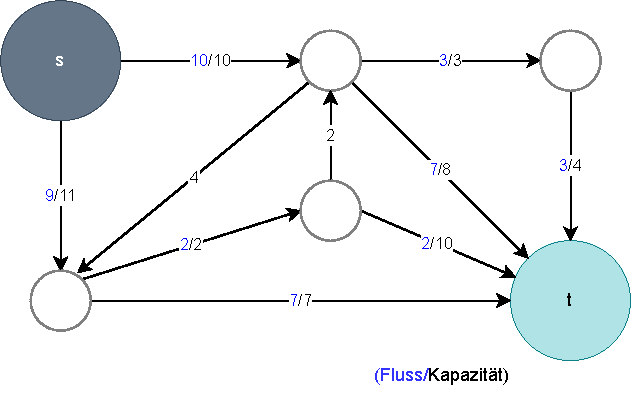
\includegraphics[width=0.7\textwidth]{img/philipp/graph1-Max Fluss.drawio.pdf}
\caption{Beispiel für maximale Flüsse}
\label{fig:maxfluss}
\end{figure}

In Abbildung \ref{fig:maxfluss} ist beispielhaft ein mögliches Maximale-Flüsse-Problem dargestellt. Jede Kante wird durch eine Kapazität und einen Flusswert beschrieben.\\
In diesem Fall hätte der maximale Fluss den Wert 19, d.h. dass in der angegebenen \textit{Kantenkonstellation} maximal 19 Einheiten zum Ziel fließen können.


\section{Definition \& Notation}

Nachdem die Vorgängerthemen nochmal wiederholt wurden, können nun die für \textit{kostenminimale Flüsse} benötigten Definitionen und Begriffe eingeführt werden.

\begin{definition}
    Sei $G = (V,E)$ ein gerichteter Graph mit oberen Kapazitäten $u(e)$ für jede Kante $e \in E$ und $b$ eine Balance. Ein b-Fluss ist eine Kantenbewertung $f(e), e \in E$, die die oberen Kapazitäten einhält und für die der Einfluss in einem Knoten $v$ abzüglich des Ausflusses in den Knoten $v$ dem Wert $b(v)$ entspricht, d.h. 
    \begin{equation}
        \displaystyle\sum_{e \in \delta ^{+} (v)}^{} f(e) - \displaystyle\sum_{e \in \delta ^{-} (v)}^{} f(e) = b(v)
    \end{equation}
\end{definition}

Die Formel der Flusserhaltung wurde somit um den Begriff der \textit{Balance} erweitert. Entsprechend gilt die Flusserhaltung bei einer Balance von Null. Durch diese Regel hat eine Quelle\footnote{welche mehr emittiert als aufnimmt} eine positive Balance und eine Senke\footnote{welche mehr aufnimmt als emittiert} eine negative Balance.

Unter Berücksichtigung des Wissens aus den \enquote{Maximalen Flüssen}, ist ein Ziel, die Balancen auf Null zu bekommen, also eine konsequente Flusserhaltung zu erzeugen. Damit dies möglich ist, kann die folgende Aussage angenommen werden:
\begin{equation*}
    \displaystyle\sum_{v \in V}^{} b(v) = 0
\end{equation*}
Diese Aussage sorgt nicht nur dafür, dass die Flusserhaltung überall eingehalten wird, sondern Angebot und Nachfrage von Quellen und Senken ausbalanciert sind.

Um die b-Flüsse untereinander vergleichen zu können, erfordert es einer neuen Metrik:

\begin{definition}
    Sei $G = (V,E)$ ein gerichteter Graph mit oberen Kapazitäten $u(e) \in \mathbb{N}$ und Kosten $c(e) \in \mathbb{Z}$ für jede Kante $e \in E$. Außerdem sei $b$ eine Balance. Ein kostenminimaler Fluss $f$ ist ein b-Fluss mit minimalen Kosten. Die Kosten eines b-Flusses sind gegeben durch
    \begin{equation}
        c(f) = \displaystyle\sum_{e \in E}^{} c(e) \cdot f(e)
    \end{equation}
\label{def:costfunktion}
\end{definition}

Anders formuliert, entsprechen Kostenminimale Wege dem kostengünstigten Weg unter Beachtung der Kapaziätsgrenzen mit dem Ziel, dass die Balancen gleich null sind.

\section{Erste Anwendung}
Angenommen, es liegt der aus dem Logistikbeispiel bekannte Graph vor (siehe Abbildung \ref{fig:baeckerbeispiel2}). In dieser Darstellung erhält jede Kante $v$ ein Kantengewicht $c(v)$ (grauer Wert) sowie eine Kapazität $f(v)$ (schwarzer Wert). Das Ziel ist es, dass bei dem mittleren Zielknoten $t2$ eine Einheit und bei den verbleibenden $t_x$ zwei Einheiten ankommen.

\begin{figure}[ht]
\centering
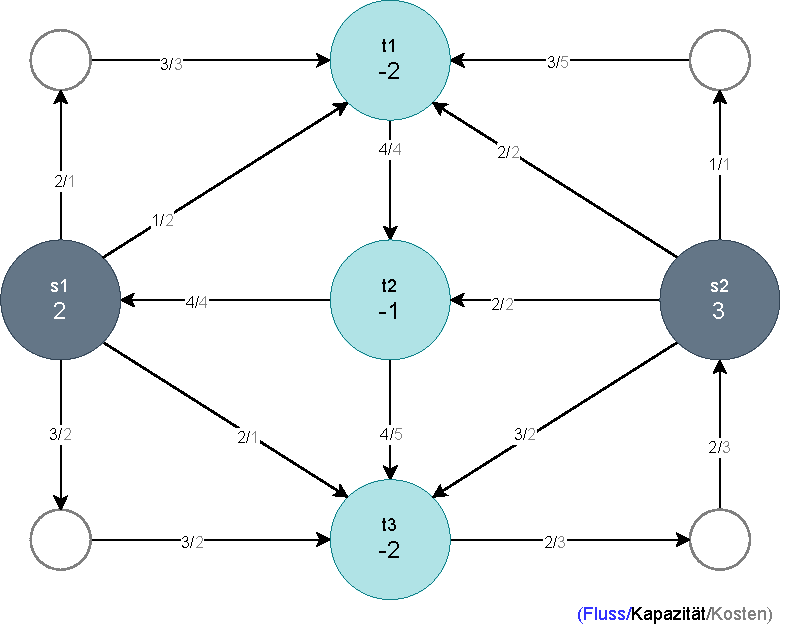
\includegraphics[width=0.7\textwidth]{img/philipp/graph1-example0.drawio.pdf}
\caption{Formelle Darstellung des Logistikbeispiels}
\label{fig:baeckerbeispiel2}
\end{figure}

Durch Ausprobieren lassen sich nun verschiedene Flüsse ermitteln, wie in den Abbildungen \ref{fig:baeckerbeispiel_loesungen1} und \ref{fig:baeckerbeispiel_loesungen2} exemplarisch zu sehen ist. Diese müssen nun lediglich auf ihr kumuliertes Kantengewicht überprüft werden. In diesem Fall hätte Möglichkeit 1 ein Gewicht von 5 und Möglichkeit 2 ein Gewicht von 6, womit die erste die \textit{kostenminimalere} ist.

\begin{figure}[htb]
\centering
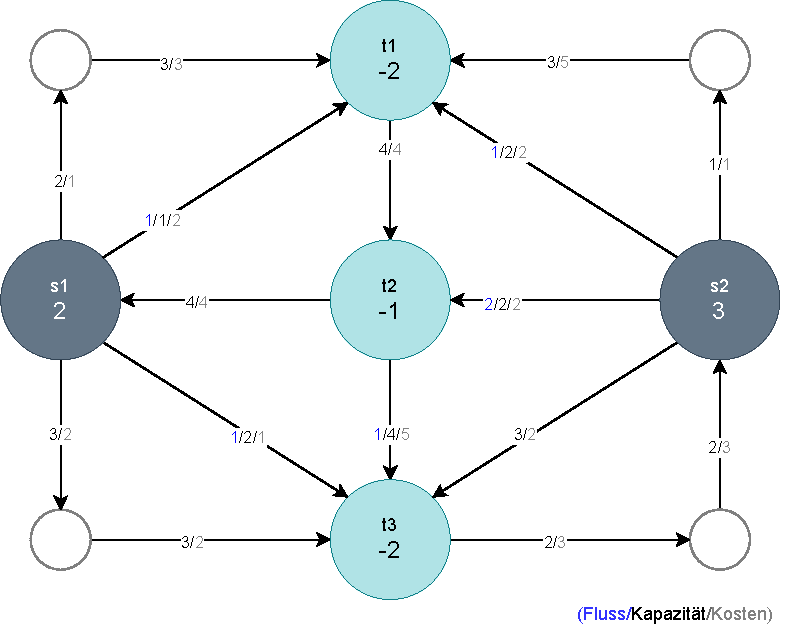
\includegraphics[width=0.7\textwidth]{img/philipp/graph1-example1.drawio.pdf}
\caption{1. Möglicher Fluss des Logistikbeispiels}
\label{fig:baeckerbeispiel_loesungen1}
\end{figure}

\begin{figure}[htb]
\centering
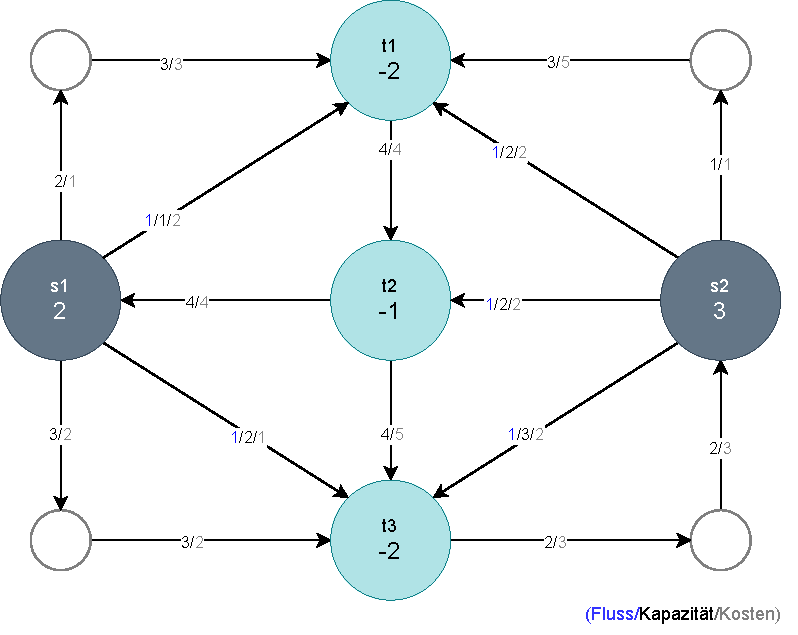
\includegraphics[width=0.7\textwidth]{img/philipp/graph1-example 2.drawio.pdf}
\caption{2. Möglicher Fluss des Logistikbeispiels}
\label{fig:baeckerbeispiel_loesungen2}
\end{figure}

Würde man nun, statt nur zwei, alle Möglichkeiten ausprobieren, wäre der Fluss mit dem geringsten Kantengewicht der gesuchte kostenminimale Fluss. \\
Bekanntermaßen ist eine Herangehensweise, in der alle möglichen Wege durchprobiert werden (vergleichbar zu \textit{BruteForce}) intuitiv, jedoch unverhältnismäßig ineffizient. Diese Ausarbeitung wird in den nächsten Kapiteln bessere Wege aufzeigen, um solche Probleme zu lösen. Hierzu wird sich eines Optimalitätskriteriums unter Anwendung der Residualgraphen bedient, die Thema des nächsten Kapitels sein werden.
\chapter{Problembeschreibung und Optimalität}

\begin{definition}[Min-Cost-Flow-Problem (im Folgenden: MCFP)]
Ziel des \textbf{MCFP} ist es, eine Flussfunktion $f$ oder auch einen $b-Fluss$ in einem Flussnetzwerk zu finden, welche(-r) eine gegebene Kostenfunktion minimiert. Dabei soll die Zielfunktion die günstigste Möglichkeit für den Transport von einem oder mehreren Startpunkten (Quellen) durch ein Netzwerk zu einem oder mehreren Zielpunkten (Senken) repräsentieren. Kapazitätsbeschränkungen als auch Balancen im Graphen sollen dabei eingehalten werden.
\end{definition}
In diesem Kapitel soll darauf eingegangen werden, anhand welchen Kriteriums ein $b-Fluss$ in einem Flussnetz als minimal/optimal betrachtet werden kann. Dabei wird zu Erklärungszwecken auf komplexe Graphen verzichtet. Zunächst aber noch ein paar Erläuterungen, welche zum Verständnis des Optimalitätskriterium benötigt werden.

\section{Prinzip der Residualgraphen}
Das Prinzip des Residualgraphen oder auch Restgraphen ist bereits aus dem \textit{Maximaler-Fluss-Problem (MFP)} bekannt. Dabei handelt es sich um eine Art \textit{Zurücksende-Prinzip}. Es basiert auf der Überlegung, dass bereits versendete Einheiten auf dem gleichen Weg, auf dem sie gesendet wurden, auch wieder zurückgesendet werden könnten. In der Modellierung wird dann zu einem vorhandenen Fluss in einem gegebenen Flussnetz ein \textit{Residualgraph} oder auch \textit{Restgraph} erstellt, welcher die entsprechenden Rücksendewege als Rückwärtskanten beinhaltet. Wichtig ist, der Residualgraph repäsentiert den möglichen Fluss, welcher verändert werden kann, deshalb werden in diesem Graphen keine Flüsse eingezeichnet.
\begin{definition}[Residualgraph]
Der \textbf{Residualgraph $G^f$} eines Flussnetzes ist ein Graph, der zusätzliche mögliche Flüsse anzeigt. Wenn es einen Pfad von der Quelle zur Senke im Residualgraphen gibt, dann ist es möglich, einen Fluss hinzuzufügen bzw. vorhandenen Fluss zu erhöhen. Jede Kante eines Residualgraphen hat einen Wert, die \textbf{Residualkapazität}(Rest-Kapazität)  \textbf{$u^f$}, welche gleich der ursprünglichen Kapazität der Kante abzüglich des aktuellen Flusses ist.
\end{definition}
\begin{figure}[htb]
\centering
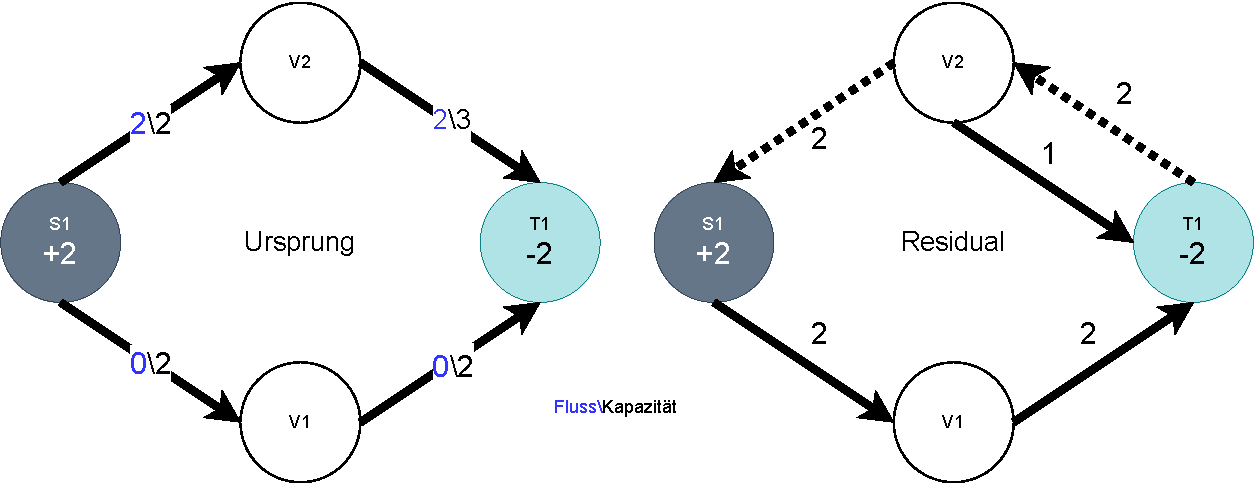
\includegraphics[width=0.9\textwidth]{img/steffen/simple_residual.drawio.pdf}
\caption{Einfacher Graph mit b-Fluss ($f1$) und korrespondierendem Residualgraph ($f1'$)}
\label{fig:simple_residual}
\end{figure}
In der Grafik \ref{fig:simple_residual} ist auf der linken Seite ein einfacher \textit{b-Fluss (S1, V2, T1)} in einem Graphen modelliert. Auf der rechten Seite ist der zugehörige Residualgraph abgebildet. Die Kanten, über die ursprünglich der \textit{b-Fluss} mit dem \textit{value=2} geflossen ist, werden nun als Rückwärtskanten dargestellt. Da auf der Kante \textit{E(V2,T1)} die Kapazität noch nicht voll ausgeschöpft ist, wird die Differenz aus Originalkapazität und vorhandenem Fluss auf der Vorwärtskante eingetragen.

\newpage
\subsection{Augmentierende Wege}
Innerhalb des Residualgraphen ist es unter Umständen möglich einen Weg von $s$ nach $t$ zu finden, über den ein Fluss > 0 gesendet werden kann, so dass der Gesamtfluss beeinflusst werden kann und weiterhin alle Kapazitätsgrenzen einhält. Ein solcher Weg wird als augmentierender Weg oder auch augmentierender Pfad bezeichnet.
\begin{definition}[Augmentierende Wege]
Ein Weg von $s$ nach $t$ im Residualgraph eines Flussnetzwerks heißt augmentierender Weg oder auch augmentierender Pfad wenn:
Der Weg von der Quelle zur Senke, entlang des Fluss weiter vergrößert(augmentiert) werden kann, ohne die Kapazitätsbeschränkungen der Kanten zu verletzen.
\end{definition}
\begin{figure}[htb]
\centering
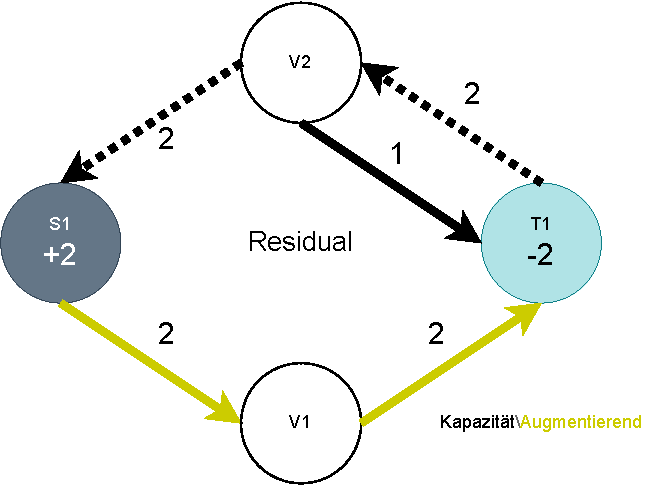
\includegraphics[width=0.7\textwidth]{img/steffen/augmented_way.drawio.pdf}
\caption{Augementierender Weg}
\label{fig:augmented_way}
\end{figure}
Die Grafik \ref{fig:augmented_way} zeigt in Gelb eingezeichnet einen augmentierenden Weg im Residualgraphen. Da im Ursprungsgraphen $G^f$ über diesen Weg noch keine Kapazitäten gesendet wurden, wäre es theoretisch möglich hier den Fluss zu erhöhen.

\subsection{Kosten}
Um das MCFP modellieren zu können, müssen Kosten abgebildet werden. Diese Kosten $c(e)$ in einem Graphen $G$ werden als Gewichtung an den Kanten dargestellt. Die Kosten können dabei exklusiv oder auch parallel zu anderen Gewichtungen existieren. Je nach Struktur der Kostenfunktion ist das zugrunde liegende Min-Cost-Flow-Problem \textit{np-hart} oder es existieren polynomiell exakte Algorithmen. Im Allgemeinen ist die Lösung von Min-Cost-Flow Problemen nicht eindeutig.
\begin{figure}[htb]
\centering
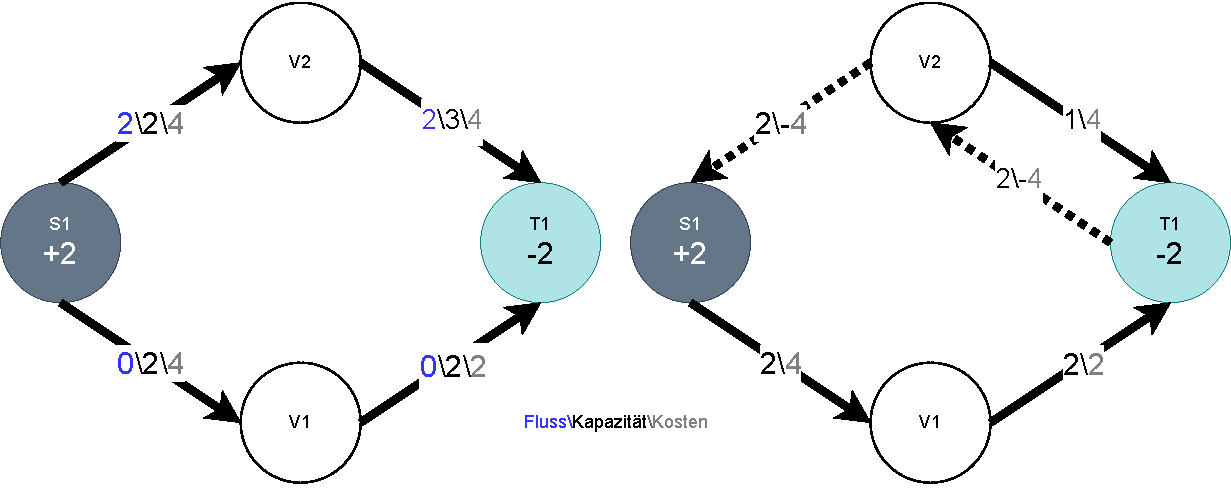
\includegraphics[width=1.0\textwidth]{img/steffen/graph_and_residual_with_costs.drawio.pdf}
\caption{Einfacher Graph mit b-Fluss($f1$), Kosten und zugehörigem Residualgraph ($f1'$)}
\label{fig:graph_and_residual_with_costs}
\end{figure}
Die Gesamtkosten von $f1$ in Abbildung \ref{fig:graph_and_residual_with_costs} entsprechen:
\begin{equation}
    f1 = 2*4 + 2*4 + 0*4 + 0*2 = 16
\end{equation}
%\textbf{Residualkosten}
\begin{definition}[Residualkosten $c^f$Satz 10.5]
Die Vorwärtskanten von Knoten im Residualgraphen bekommen die ursprünglichen Kosten zugewiesen und die Rückwärtskanten den negativen Wert ihrer Vorwärtskanten:
\begin{equation}
    \forall e \in E \quad c^f (e) = c(e) \Leftrightarrow c^f (\overleftarrow{e}) = -c(e)
\end{equation}
\end{definition}
Abbildung \ref{fig:graph_and_residual_with_costs} zeigt neben dem Originalgraphen auch den Residualgraphen mit bereits eingetragenen Kosten. Über die Kanten (S1, V2) und (V2, T1) fließt $b$ im Originalgraphen. Deshalb erhalten die Rückwärtskanten negative Kosten, die Vorwärtskanten behalten die originalen positiven Kosten.

\section{Lösung des MCFP mit Ford-Fulkerson?}

\textbf{Kann das MCFP durch den Ansatz von Ford-Fulkerson gelöst werden?} Sprich:
Kann durch sukzessives Erhöhen des Flusses mit Hilfe von (s-t)-Wegen aus dem Residualgraphen ein optimales Ergebnis für das MCFP gefunden werden? Welche Rolle spielt dabei die Kostenfunktion? Zunächst hier noch ein kurzer Rückblick auf die Optimalität von MFP:

\subsection{Optimalität von maximalen Flüssen}

Für das MFP war das Ziel in einem gegebenen Flussnetz (mit einer endlichen Menge an (s-t)-Flüssen) mindestens einen auszuwählen, für den die aus $s$ ausgehenden Flussmengen abzüglich der eingehenden Flussmengen maximal sind. Für diesen Fluss gilt das MFP als optimal. Formal ausgedrückt ist Kriterium für die Optimalität des MFP:
\begin{definition}[Satz 10.5]
    Ein (s, t)-Fluss $f$ oder auch b-Fluss ist genau dann maximal, wenn es \textbf{\textit{keinen f-augmentierenden Weg in $G^f$}} gibt. Dabei entspricht $G^f$ dem Residualgraphen.
\end{definition}
Mit anderen Worten: Erhöhe den Fluss in einem Graphen solange, bis aus dem Residualgraphen hervorgeht, dass keine weitere Flusserhöhung möglich ist.

\subsection{Augmentierende Wege und b-Flüsse}

Erwiesen ist, dass ein gegebener \textbf{(s-t)-Fluss} in einem Flussnetz systematisch verändert bzw. umgeleitet werden kann, ohne dabei Kapazitätsbeschränkungen zu verletzen. Das heißt auch, dass es möglich sein muss in einem Graphen für beliebige \textbf{(s-t)-Flüsse} einen auszuwählen, welcher ein zulässiger Fluss sein muss, aber auch möglichst niedrige Kosten haben kann. Aber gilt:
\begin{equation}
    \textbf{Maximaler-Fluss} = \textbf{b-Fluss} ???
\label{formular:st_flow_eq_b_flow}
\end{equation}

Schaubild \ref{fig:augmented_way} enthält einen f-augmentierenden Pfad durch den Residualgraphen $G^f$. Nach dem Vorgehen von Ford-Fulkerson würde der Fluss nun in einem resultierenden Graphen um 2 über den Weg (S1,V1,T1) erhöht werden.
\begin{figure}[htb]
\centering
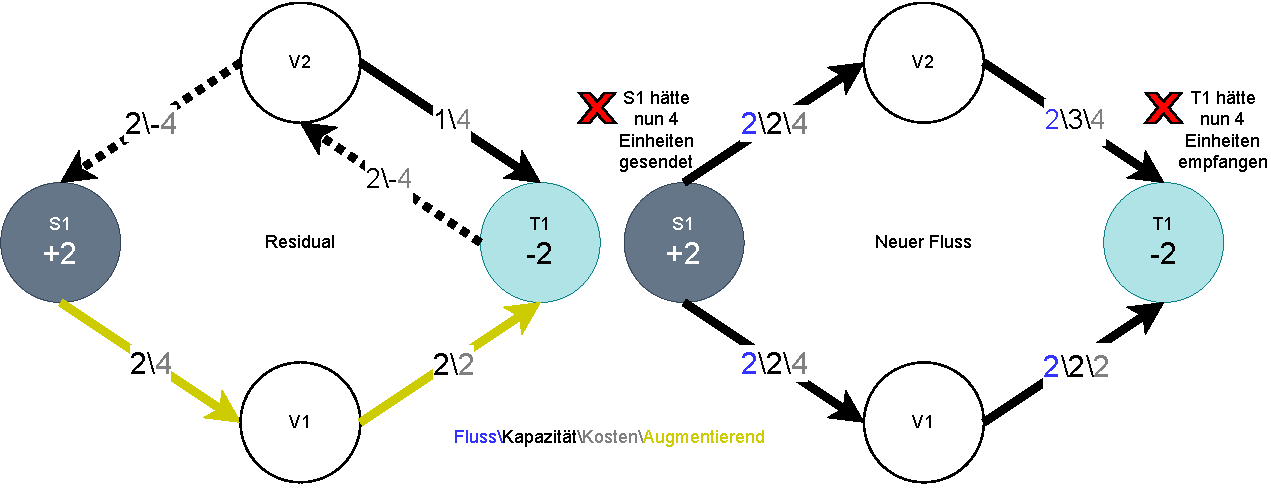
\includegraphics[width=1.0\textwidth]{img/steffen/augmented_way_with_resulting.drawio.pdf}
\caption{Residualgraph ($f1'$) mit augmentierendem Weg und resultierender Fluss ($f2$)}
\label{fig:augmented_way_with_resulting_graph}
\end{figure}
In der Veranschaulichung \ref{fig:augmented_way_with_resulting_graph} ist zu erkennen, dass direkt mehrere Probleme aus diesem Vorgehen entstehen:
\begin{itemize}
\item Weder die Balance von S1 noch T1 werden in $f2$ eingehalten
\item $c(f2)$ = \textbf{30 > 16} = $c(f1)$
\end{itemize}
Daraus lässt sich folgern, dass gilt:
\begin{equation}
    \textbf{Maximaler-Fluss} \neq \textbf{b-Fluss} !!!
\label{formular:st_flow_neq_b_flow}
\end{equation}
Weiterhin fällt es nicht schwer zu erkennen, dass die naive Anwendung von augmentierenden Pfaden nicht zu einer optimalen Lösung des MCFP führt.

\subsection{Kürzeste Wege und b-Flüsse}

Würde der ursprüngliche Fluss aus $f1$ über (S1, V2, T1) in Abbildung \ref{fig:invalid_b_flow} wegfallen, so wären die Balancen im Graphen wieder eingehalten und die resultierenden Kosten von $f2$ würden auf 12 sinken und damit wäre $c(f2)$ < $c(f1)$. Hinsichtlich der Forderung des MCFP nach minimalen Kosten wäre diese Option auf jeden Fall besser. Für den gegebenen Graphen ist dies sogar der optimale b-Fluss.
\begin{figure}[htb]
\centering
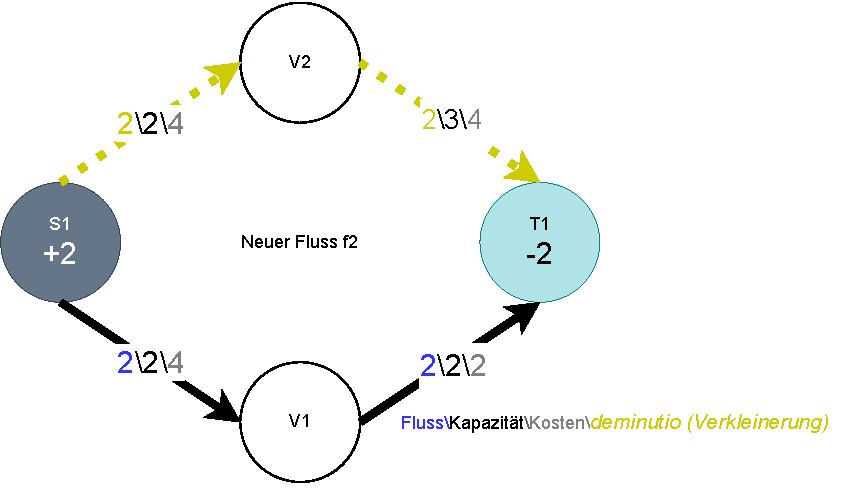
\includegraphics[width=0.6\textwidth]{img/steffen/invalid_b_flow.drawio.pdf}
\caption{(s-t)Fluss ($f2$) mit Weg, welcher die Balancen im Graphen verletzt.}
\label{fig:invalid_b_flow}
\end{figure}
Losgelöst kann der Minimale Kostenfluss in einem Graphen auch als kürzester Weg von $s$ nach $t$ bezüglich der Kosten betrachtet werden. Ein Pfad/Weg von $s$ nach $t$ ist genau dann ein kürzester Weg, wenn seine Gesamtkosten minimal sind. Gesucht ist also der Shortest Cost Flow $f$ in G, welcher im Graphen \ref{fig:invalid_b_flow} bereits in blau eingezeichnet ist. Es muss nur noch der gelbe Ursprungsfluss wieder zurück geleitet werden.
\begin{figure}[htb]
\centering
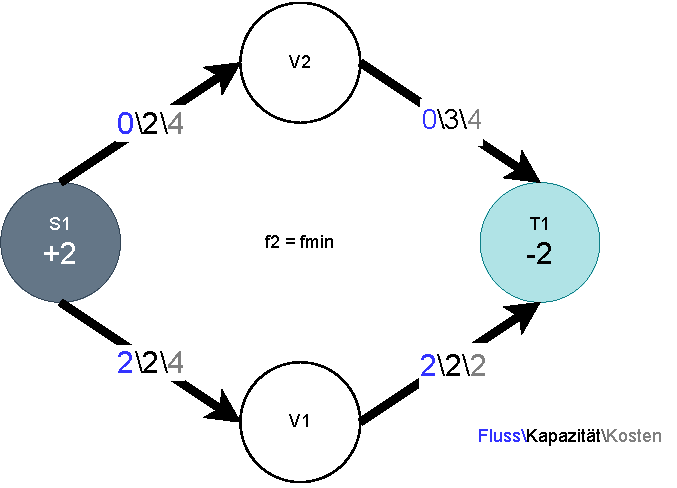
\includegraphics[width=0.6\textwidth]{img/steffen/min_cost_flow_graph.drawio.pdf}
\caption{$f2$ als Minimaler Kostenfluss in $G$}
\label{fig:min_cost_flow_graph}
\end{figure}
In dem Graphen \ref{fig:min_cost_flow_graph} ist der minimale Kostenfluss für das gegebene Flussnetz ohne den ursprünglichen Fluss eingetragen. Alle Bedingungen sind erfüllt. \textbf{Warum ist dies nun die optimale Lösung?}

\section{Augmentierende Zykel und Optimalität}

In der Gegenüberstellung der Residualgraphen von f1 und f2 (Abbildung \ref{fig:resi_f1_vs_f2}) sind jeweils zwei Zykel farblich hinterlegt.
\begin{definition}[Augmentierende Zykel]
Statt eines f-augmentierenden Wegs, der für maximale Flüsse benötigt wird, definieren wir nun einen f-augmentierenden Zykel Z. Ein f-augmentierender Zykel ist ein gerichteter Kreis in dem Residualgraphen $G^f$
\label{def:augmented_cycle}
\end{definition}
\begin{figure}[htb]
\centering
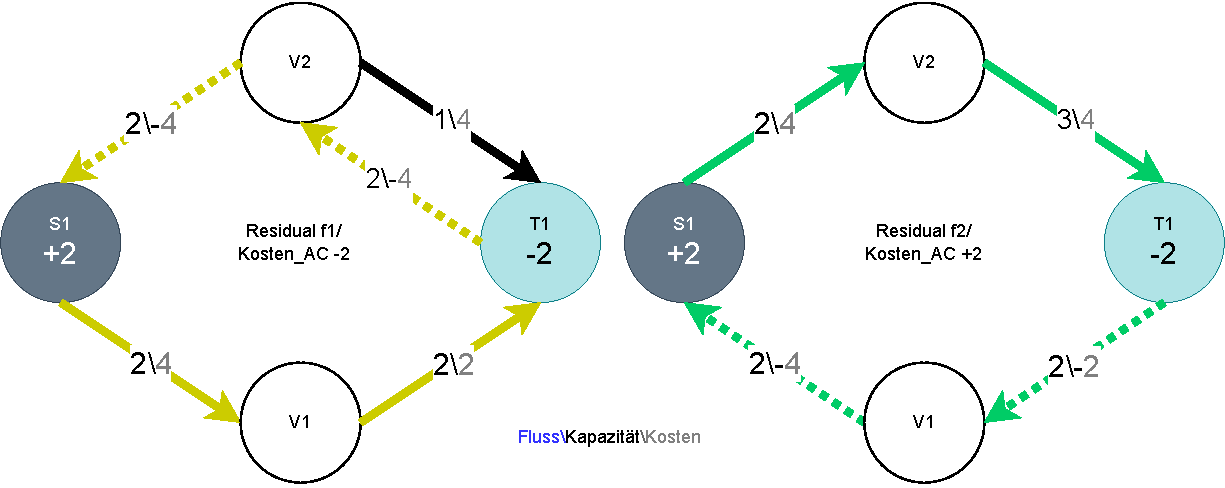
\includegraphics[width=1.0\textwidth]{img/steffen/resi_f1_vs_f2.drawio.pdf}
\caption{Residualgraph zu $f1$ gegenüber Residualgraph $f2$}
\label{fig:resi_f1_vs_f2}
\end{figure}
Summiert ergeben die Kosten entlang der farblich markierten Zykel jeweils \textit{c(f1') = -2} und \textit{c(f2') = 2}. Daraus lässt sich folgendes Vermuten (der formale Beweis der Optimalität wird hier aus Komplexitätsgründen bewusst ausgeklammert. Es darf davon ausgegangen werden, dass das Optimalitätskriterium gilt):

\begin{definition}[Satz 11.1 (Optimalitätskriterium für MCFP, Klein 1967).]
    Sei $G = (V, E)$ ein gerichteter Graph, $u$ die oberen Kantenkapazitäten, $c$ eine Kostenfunktion auf den Kanten und $b$ eine Balance. Dann ist $f$ genau dann ein kostenminimaler Fluss, wenn kein f-augmentierender Zykel $Z$ mit negativen Kosten in $G^f$ existiert.
\end{definition}

\subsection{Wie findet man negative Zykel?}

Um in einem Graphen einen minimalen Kostenfluss zu finden, ist es also essentiell Möglichkeiten bzw. Algorithmen zu haben, welche Zykel in Graphen erkennen können. Hier eine (nicht vollständige) Auflistung:

\begin{itemize}
\item \textbf{Moore-Bellman-Ford-Algorithmus O(n*m)}
\item Robust-Dijkstra-Algorithmus O(n*m)
\item Goldberg-Radzik-Algorithmus O(n*m)
\end{itemize}

Es fällt auf, dass es laut dieser Liste keinen Algorithmus gibt, welcher eine Komplexität von O(n*m) unterschreitet. Wurde ein negativer Zykel in einem Residualgraphen gefunden, kann dann durch Augmentieren eines b-Fluss $b1$ um den Wert $\gamma$  ein neuer b-Fluss $b2$ erzeugt werden, welcher den gefundenen Zykel nicht mehr beinhaltet.
\begin{equation}
    \gamma \leq min_{e\in Z} u^f(e)
\label{def:gamma}
\end{equation}
Es kann sein, dass der neue $b-Fluss$ weitere negative Zykel beinhaltet. Diese können dann iterativ aufgelöst werden. Bis kein weiterer Zykel mehr vorhanden ist (siehe auch: Cycle cancelling algorithm):

\[ f'(e) = \begin{cases}
 f(e) & \text{falls } e \notin Z \\
 f(e) + \gamma & \text{falls    } e \in Z\\
 f(e) - \gamma & \text{falls    } \overleftarrow{e} \in Z
\end{cases} \]
Bezogen auf Abbildung \ref{fig:resi_f1_vs_f2} bedeutet das, durch die Erhöhung des augmentierenden Zyklus in f1' um den Wert 2 entsteht f2. Der daraus resultierende Residualgraph f2' enthält nach der Augmentierung einen positiven Zykel.

\subsection{Welche Algorithmen lösen ein MCFP?}

Stand 2022-Mai sind diverse Algorithmen bekannt, welche das MCFP lösen können. Ein paar davon sind hier aufgelistet. 

\begin{itemize}
 \item \textbf{Cycle cancelling algorithm (negative cycle optimality)}
 \item \textbf{Successive Shortest Path algorithm (reduced cost optimality)}
 \item Out-of-Kilter algorithm (complimentary slackness)
 \item Push/Relabel algorithm
 \item Dual Cancel and Tighten
 \item Primal-Dual
\end{itemize}

Die ersten beiden werden in den folgenden Kapiteln näher betrachtet.


% \textbf{Exkurs}
% Die Anwendung des Lagrange-Multiplikator hat sich als nicht praktikabel erwiesen.
% \textit{Lineare Kostenfunktion}
% \begin{itemize}
%     \item Linear Programing
%     \item Simplex Algorithm
% \end{itemize}
% \textit{Konvexe Kostenfunktion}
% \begin{itemize}
%     \item Capacity-Scaling Algorithm --> Linearisierung
% \end{itemize}
% \textit{Allgemeine nichtlineare Kostenfunktion}
% \begin{itemize}
%     \item Für allgemeine nichtlineare Kostenfunktionen ist das Finden einer Lösung in einem Min-Cost-Flow-Problem NP-schwer.
% \end{itemize}
\chapter{Cycle-Canceling-Algorithmus}
Für das Maximale-Fluss-Problem existiert der Ford-Fulkerson Algorithmus, welchen wir bereits kennengelernt haben. Dieser Algorithmus kann so angepasst werden, dass dieser auch für die Berechnung eines kostenminimalen Flusses benutzt werden kann. Die Anpassung sieht wie folgt aus: Anstatt mit einem $(s, t)$-Fluss zu starten, beginnt man mit einem $b$-Fluss. Nun berechnet man in jeder Iteration einen $f$-augmentierten Zykel mit negativen Kosten, wodurch man als Ergebnis einen kostenminimalen Fluss bekommt. Der Algorithmus, der genau dieses Prinzip verwendet, ist der Cycle-Canceling-Algorithmus.

\begin{table}[h!]
\setlength{\tabcolsep}{20pt}
\centering
\begin{tabular}{p{2.5cm} >{\setstretch{1.5}}p{10cm}}
\toprule
\multicolumn{2}{l}{\textbf{Cycle-Canceling-Algorithmus}} \\ \midrule
%\onehalfspacing
Input:          &Gerichteter Graph G = (V, E), obere Kapazitäten u, Kantenkosten c, Balance b.\\
 ~ & ~ \\
Output:         &Kostenminimaler Fluss f .\\
 ~ & ~ \\
Schritt 1:      &Berechnen Sie einen b-Fluss.\\
Schritt 2:      &Bestimmen Sie $G^f$ , $u^f$ und $c^f$ .\\
Schritt 3:      &Konstruieren Sie einen f -augmentierenden Zykel $Z$ in $G^f$ mit negativen Kosten. Falls keiner existiert: STOPP.\\
Schritt 4:      &Verändern Sie den b-Fluss $f$ entlang des Zykels $Z$ um $\gamma := min_{e \epsilon Z} u^f (e)$.\\
Schritt 5:      &Gehen Sie zu Schritt 2 \\
                &              \\ \bottomrule  
\end{tabular}
\label{tab: cycle_canceling_algorithmus}
\caption{Cycle-Canceling-Algorithmus}
\end{table}

\section{Berechnung eines Beispielgraphen mit dem Cycle-Canceling-Algorithmus}

Im Folgenden wird die Berechnung eines kostenminimalen Flusses $f$ anhand des Beispielgraphen in Abbildung \ref{fig:cc_step1} beschrieben.
\begin{figure}[htb]
\centering
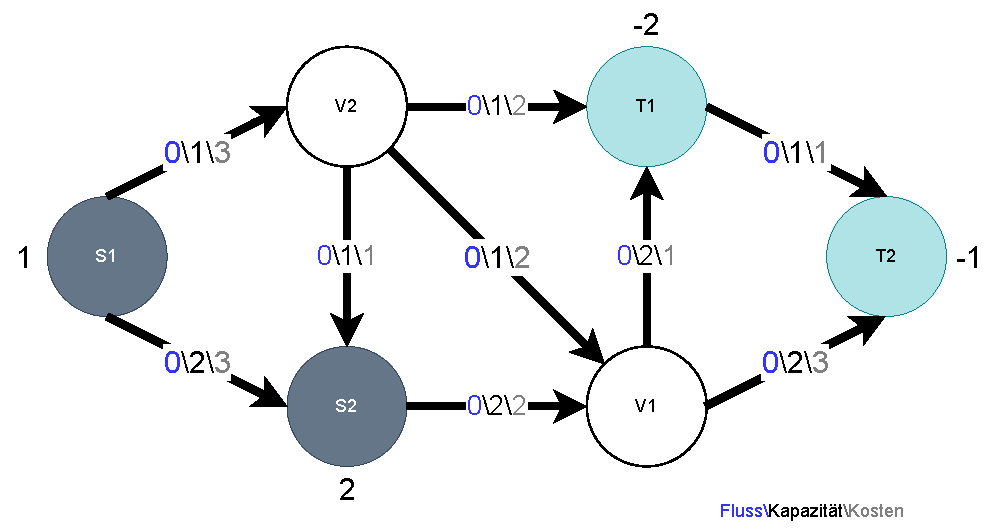
\includegraphics[width=0.7\textwidth]{img/leo/graph1-Page-1.drawio.pdf}
\caption{Cycle-Canceling-Algorithmus Schritt 1}
\label{fig:cc_step1}
\end{figure}

Im ersten Schritt des Cycle-Canceling-Algorithmuses wird ein gültiger $b$-Fluss berechnet (vgl. Abbildung \ref{fig:cc_step2}).
\begin{figure}[htb]
\centering
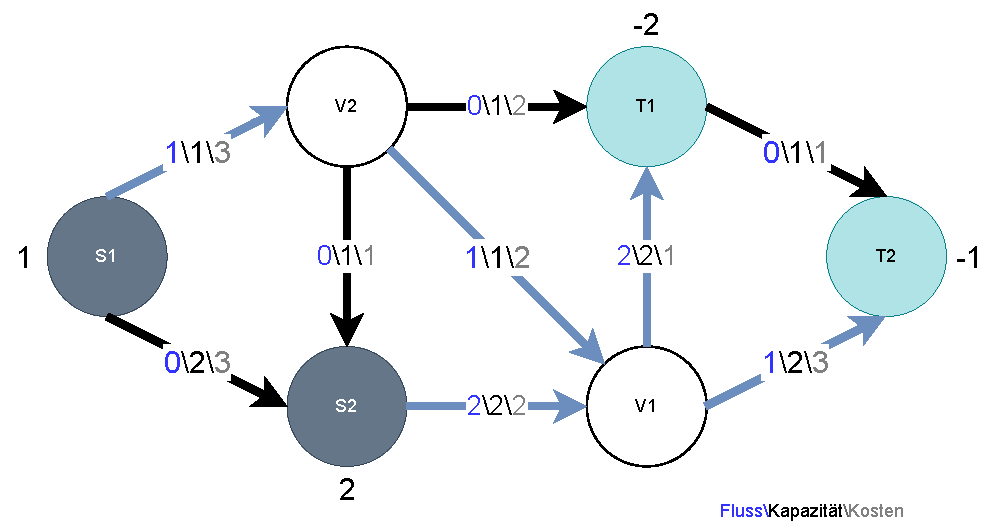
\includegraphics[width=0.7\textwidth]{img/leo/graph1-Page-2.drawio.pdf}
\caption{Cycle-Canceling-Algorithmus Schritt 2}
\label{fig:cc_step2}
\end{figure}

Im nächsten Schritt erzeugen wir zu dem in Schritt 1. bestimmten Graphen den Residualgraph mit $u^f$ und $c^f$ (vgl. Abbildung \ref{fig:cc_step3}).
\begin{figure}[htb]
\centering
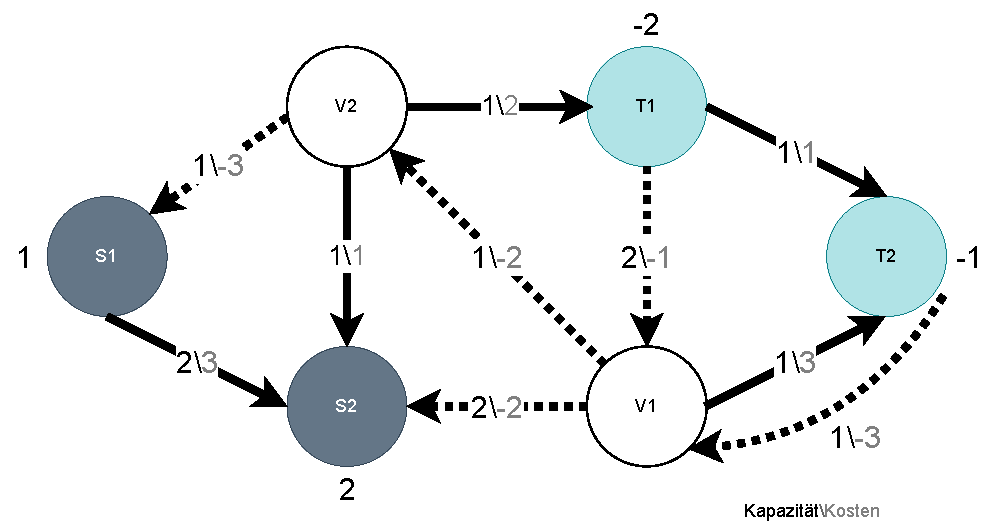
\includegraphics[width=0.7\textwidth]{img/leo/graph1-Page-3.drawio.pdf}
\caption{Cycle-Canceling-Algorithmus Schritt 3}
\label{fig:cc_step3}
\end{figure}

In Schritt 3. betrachten wir den Residualgraphen mit $u^f$ und $c^f$ und suchen in diesem nach einem Zykel, der negative Kosten hat. Gibt es keinen, sind wir mit unsrem Algorithmus fertig. In unserem Beispiel wird jedoch ein negativer Zykel mit den Kosten $-1$ von den Kanten zwischen den Knoten $V1$, $V2$ und $T1$ gebildet (vgl. Abbildung \ref{fig:cc_step4}).
\begin{figure}[htb]
\centering
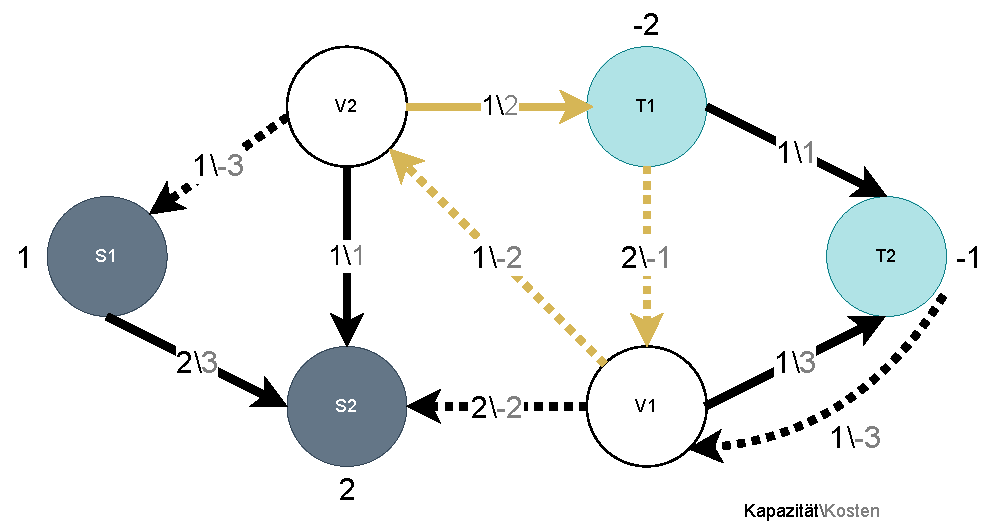
\includegraphics[width=0.7\textwidth]{img/leo/graph1-Page-4.drawio.pdf}
\caption{Cycle-Canceling-Algorithmus Schritt 4}
\label{fig:cc_step4}
\end{figure}

In Schritt 4. passen wir nun mithilfe dieses negativen Zykles unseren $b$-Fluss aus Abbildung \ref{fig:cc_step2} an. Um die Anpassung vorzunehmen, müssen wir erst die minimale Kapazität der Kanten in unserem Zykel finden. Diese minimale Kapazität ist unser $\gamma$. In unserem Fall ist $\gamma = 1$. Nun gilt haben wir im Residualgraphen eine Rückwärtskante für den Zykel benutzt, so ziehen wir unser $\gamma$ von Flusswert im ursprünglichen Graphen ab. Haben wir eine Vorwärtskante benutzt, so erhöhen wir unseren Flusswert im ursprünglichen Graphen um $\gamma$. Allgemein gilt die Definition \ref{def:augmented_cycle}. Der in unserem Beispiel entstehende Graph ist in Abbildung \ref{fig:cc_step5} zu sehen.
\begin{figure}[htb]
\centering
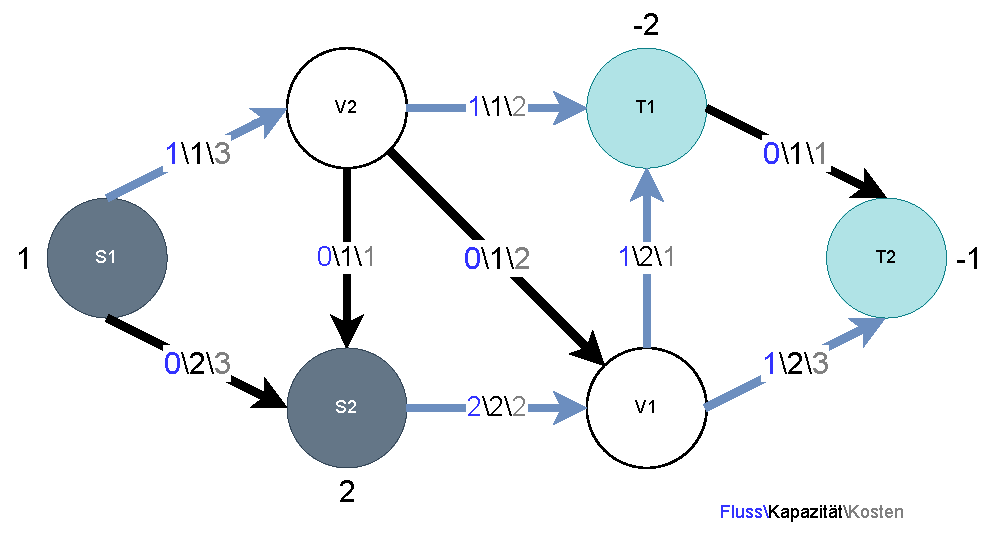
\includegraphics[width=0.7\textwidth]{img/leo/graph1-Page-5.drawio.pdf}
\caption{Cycle-Canceling-Algorithmus Schritt 5}
\label{fig:cc_step5}
\end{figure}

Zu dem neu erzeugten Graphen aus Schritt 4. wiederholen wir nun Schritt 2. Wir erzeugen erneut den Residualgraph mit $u^f$ und $c^f$ (vgl. Abbildung \ref{fig:cc_step6}).
\begin{figure}[htb]
\centering
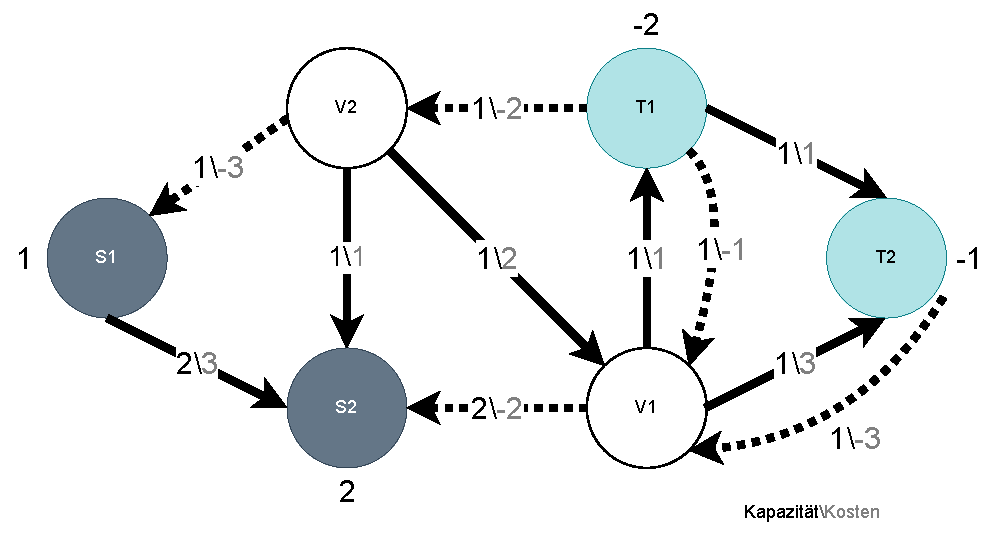
\includegraphics[width=0.7\textwidth]{img/leo/graph1-Page-6.drawio.pdf}
\caption{Cycle-Canceling-Algorithmus Schritt 6}
\label{fig:cc_step6}
\end{figure}

Nun gehen wir wieder zu Schritt 3. über und versuchen einen $f$-augmentierenden Zykel $Z$ in $G^f$ mit negativen Kosten zu konstruieren. In unserem Beispiel ist der neue Zykel nun bildbar mit den Kanten zwischen den Knoten von $T1$, $T2$ und $V1$. Der Zykel hat die Kosten $-1$ (vgl. Abbildung \ref{fig:cc_step7}).
\begin{figure}[htb]
\centering
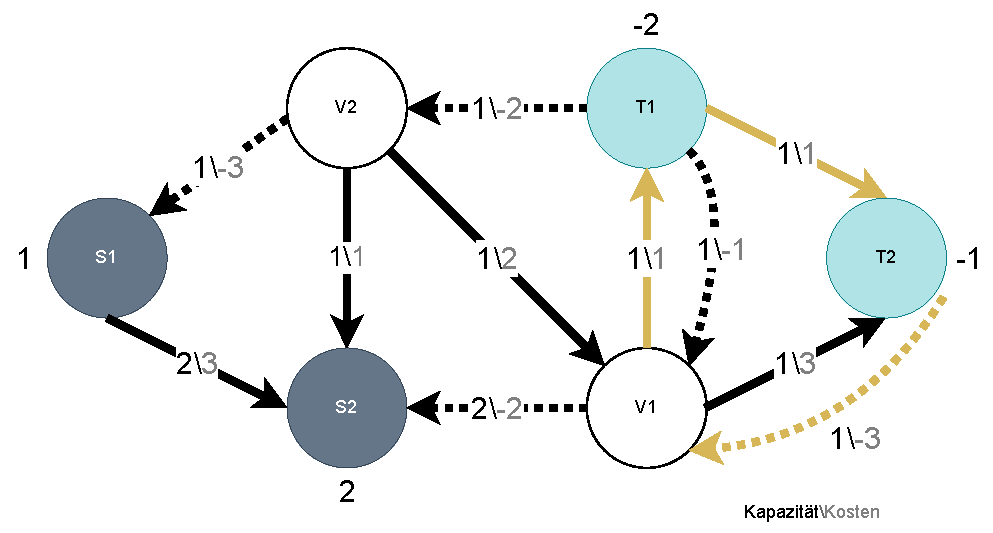
\includegraphics[width=0.7\textwidth]{img/leo/graph1-Page-7.drawio.pdf}
\caption{Cycle-Canceling-Algorithmus Schritt 7}
\label{fig:cc_step7}
\end{figure}

Im nächsten Schritt können wir nun wieder unseren ursprünglichen $b$-Fluss verändern. Dies tun wir wieder entlang des Zykels $Z$ um $\gamma := min_{e \epsilon Z} u^f (e)$. Der in unserem Beispiel neue entstehende $b$-Fluss ist in Abbildung \ref{fig:cc_step8} zu sehen.
\begin{figure}[htb]
\centering
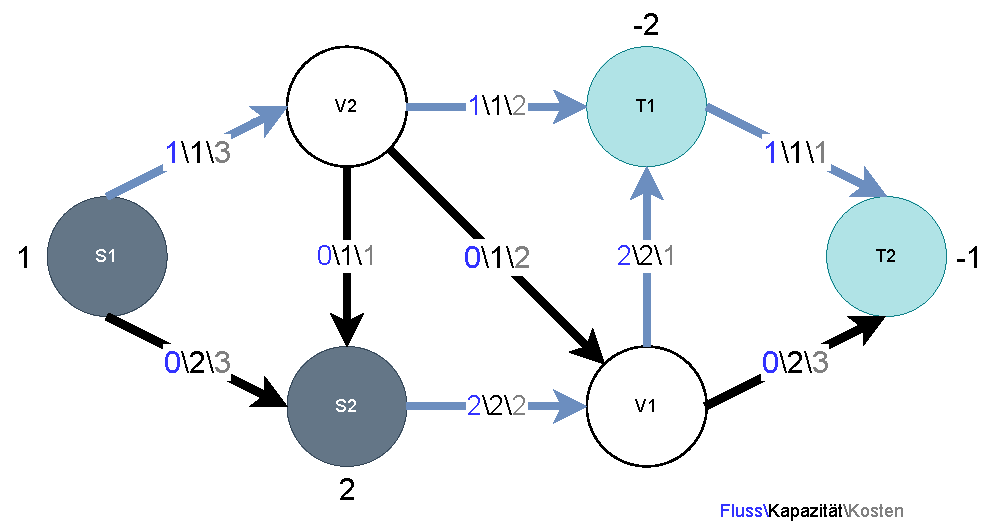
\includegraphics[width=0.7\textwidth]{img/leo/graph1-Page-8.drawio.pdf}
\caption{Cycle-Canceling-Algorithmus Schritt 8}
\label{fig:cc_step8}
\end{figure}

Nun springen wir wieder zu Schritt 2 und erzeugen den Residualgraph mit $u^f$ und $c^f$ zu dem vorigen Graphen (vgl. Abbildung \ref{fig:cc_step9}).
\begin{figure}[htb]
\centering
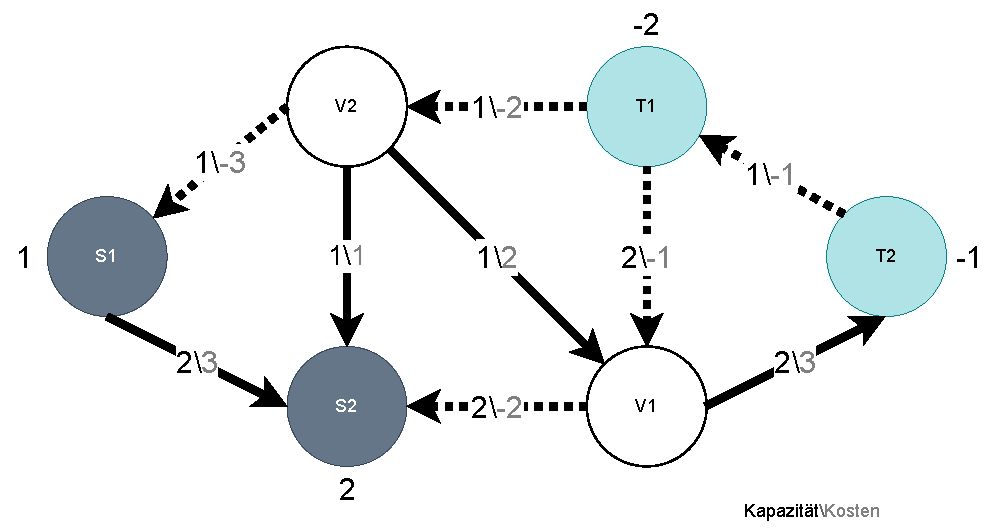
\includegraphics[width=0.7\textwidth]{img/leo/graph1-Page-9.drawio.pdf}
\caption{Cycle-Canceling-Algorithmus Schritt 9}
\label{fig:cc_step9}
\end{figure}

Danach gehen wir wieder zu Schritt 3. über wo wir versuchen, einen $f$-augmentierenden Zykel $Z$ in $G^f$ mit negativen Kosten zu konstruieren. In unserem Beispiel ist kein $f$-augmentierender Zykel $Z$ mit negativen Kosten zu konstruieren. Daraus folgt das wir unseren Algorithmus stoppen, da wir fertig sind. Unser $b$-Fluss ist nun kostenminimal.

\section{Problem des Algorithmus}
Für den Cycle-Canceling-Algorithmus ergibt sich ein ähnliches Problem, welches wir auch schon bei dem Ford-Fulkerson Algorithmus erkannt haben: Die Kosten des kostenminmalen Flusses verbessern sich im schlechtesten Fall immer nur um eine Einheit pro Iteration.

Dieses Problem können wir erneut am Diamantengraphen betrachten. Der Graph hat die Balancen $b(s) = 2N$, $b(t) = -2N$ und $b(v) = 0$. Die oberen Kapazitäten haben alle den Wert $N$ ausgenommen die Kante von $V1$ zu $V2$. Diese Kante hat die obere Kapazität $1$. Die Kosten aller Kanten betragen $0$. Nun erweitern wir den Diamantengraphen noch um eine Kante von $S$ zu $T$. Diese Kante hat die Kosten $1$ und die obere Kapazität $2N$ (vgl. Abbildung \ref{fig:erweiterter_diamantgraph}).

Das Problem wird nun ersichtlich, wenn der Algorithmus im ersten Schritt einen $b$-Fluss erzeugt, für den gilt:
\[ f(e) = \begin{cases}
 2N & $für $ e = (S,T) \\
 0 & $sonst.$
\end{cases} \]

\begin{figure}[htb]
\centering
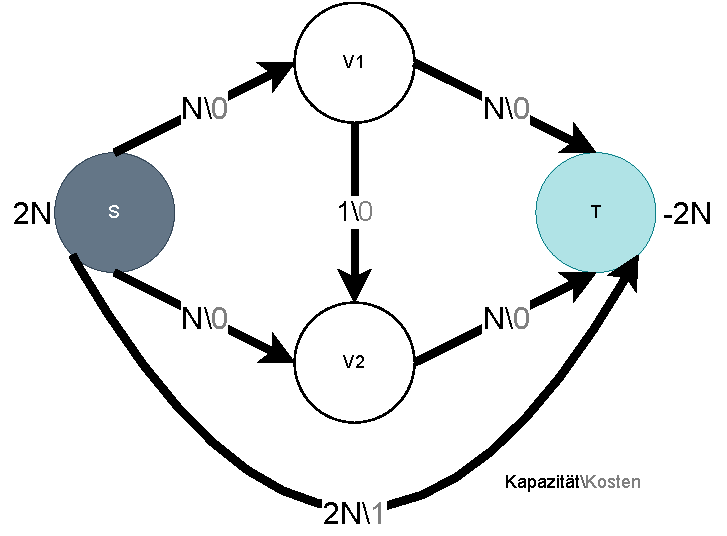
\includegraphics[width=0.7\textwidth]{img/leo/graph1-Page-10.drawio.pdf}
\caption{Erweiterter Diamantgraph}
\label{fig:erweiterter_diamantgraph}
\end{figure}

Anhand des $b$-Fluss (vgl. Abbildung \ref{fig:erweiterter_diamantgraph_mit_fluss}) kann man nun einen Zykel im Residualgraphen erzeugen, sodass mit jeder Iteration sich die Kosten des $b$-Flusses nur um eine Einheit verbessern würden. (vgl. Abbildung \ref{fig:erweiterter_diamantgraph_mit_fluss_res})

\begin{figure}[htb]
\centering
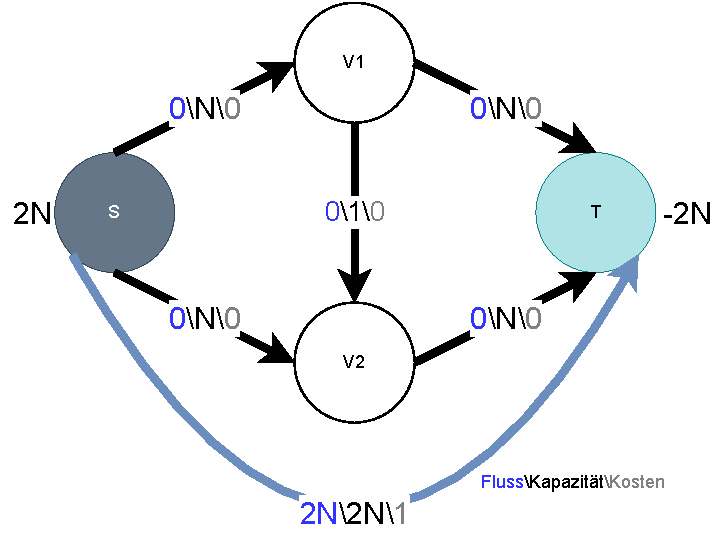
\includegraphics[width=0.7\textwidth]{img/leo/graph1-Page-11.drawio.pdf}
\caption{Erweiterter Diamantgraph mit $b$-Fluss}
\label{fig:erweiterter_diamantgraph_mit_fluss}
\end{figure}

\begin{figure}[htb]
\centering
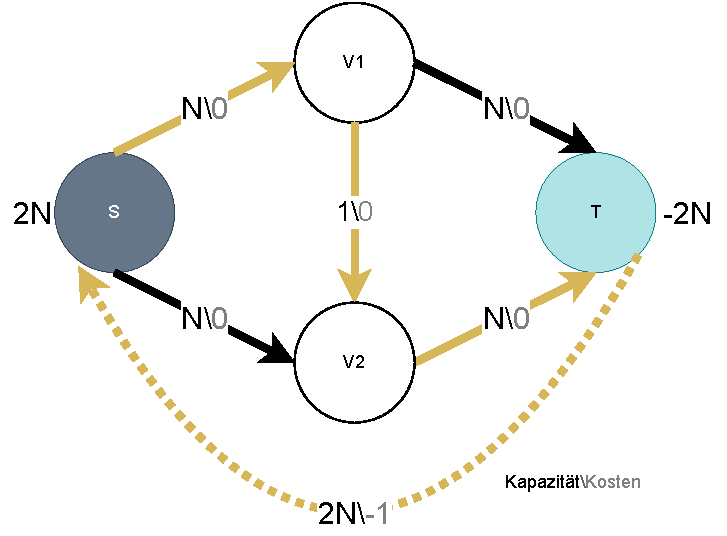
\includegraphics[width=0.7\textwidth]{img/leo/graph1-Page-12.drawio.pdf}
\caption{Residualgraph des erweiterten Diamantgraphen}
\label{fig:erweiterter_diamantgraph_mit_fluss_res}
\end{figure}


\section{Verbesserung des Algorithmus}

Eine Idee, den Algorithmus zu verbessern, wäre bei der Konstruktion des $f$-augmentierten Zykels $Z$ in $G^f$ den Zykel zu konstruieren, der die geringsten Kosten hat. Das Problem, welches sich hierbei jedoch ergibt ist, dass dies dem Problem entspricht einen Hamilton-Kreis zu finden. Eine andere Möglichkeit, die sich deshalb aufgrund der besseren Effizienz anbietet ist, dass man den Zykel mit den geringsten durchschnittlichen Kosten pro Kante wählt. Auch wenn dies schlechter ist als den Zykel mit den geringsten Kosten zu wählen.
\chapter{Succesive-Shortest-Path-Algorithmus}
Im folgenden Kapitel wird ein Blick auf einen weiteren Algorithmus geworfen, der verwendet werden kann, um einen kostenminimalen Fluss zu erzeugen.
\section{Einleitung}
Der Successive-Shortest-Path-Algorithmus (im folgenden SSPA) verwendet einen anderen Ansatz als der Cycle-Cancelling-Algorithmus. Der Cycle-Cancelling-Algorithmus benötigt als Input einen Graphen in dem ein $b$-Fluss möglich ist. Nachdem dieser berechnet ist spielt die Balance keine Rolle mehr. Denn sofern ein $b$-Fluss existiert muss immer eine Balance existieren. %ist das wirklich so?
Im Successive Shortest Path wird zunächst nicht auf den $b$-Fluss geschaut. Stattdessen wird darauf abgezielt solange günstige Wege zu finden bis alle Knoten ausbalanciert sind.

\section{Formaler Aufbau}
\begin{table}[H]
    \setlength{\tabcolsep}{20pt}
    \centering
    \begin{tabular}{p{2.5cm} >{\setstretch{1.5}}p{10cm}}
    \toprule
    \multicolumn{2}{l}{\textbf{Successive-Shortest-Path-Algorithmus}} \\ \midrule
    %\onehalfspacing
    Input:          & Gerichteter Graph $G = (V, E)$, obere Kapazitäten $u$, Kantenkosten $c$, Balance $b$.         \\
     ~ & ~ \\
    Output:         & Kostenminimaler Fluss $f$, falls existent, oder Aussage, dass keiner existiert.                \\
     ~ & ~ \\
    Schritt 1:      & Setzen Sie
       \[ f(e) = \begin{cases}
         0 & \text{falls } c(e) \ge 0 \\
         u(e) & \text{falls } c(e) < 0 
       \end{cases} \]
    und
    \begin{equation*}
        b'(v) = \displaystyle\sum_{e \in \delta ^{+} (v)}^{} f(e) - \displaystyle\sum_{e \in \delta ^{-} (v)}^{} f(e).
    \end{equation*}\\
    Schritt 2:      & Wählen Sie einen Knoten $s$ mit $b(s) - b'(s) > 0$ als Quelle und einen Knoten $t$ mit $b(t) - b'(t) < 0$ als Senke. Der Knoten $t$ muss vom Knoten $s$ im Residualgraph $G^f$ erreichbar sein. Dann gehen Sie zu Schritt 3. Existiert kein solches Paar aus $s$ und $t$ und $b(v) = b'(v)$ gilt für alle $v \in V$, dann ist $f$ kostenminimal. Ansonsten gibt es keinen $b$-Fluss.              \\
     ~ & ~ \\
    Schritt 3:      & Berechnen Sie einen kürzesten Weg $p$ bzgl. $c^f$ in $G^f$.               \\
     ~ & ~ \\
    Schritt 4:      & Verändern Sie den $b$-Fluss entlang des Weges p um den minimalen Wert aus Kapazität, Quelle und Senke:
    \begin{equation*}
        \gamma := min\{\underset{e \in p}{min} \{u^f (e) \}, b(s) - b'(s), b'(t) - b(t)\}.
    \end{equation*}              \\
     Schritt 5:     & Gehen Sie zu Schritt 2.              \\
                    &              \\ \bottomrule  
    \end{tabular}
\caption{Formaler Ablauf Successive-Shortest-Path}
\label{tab:form_sspa}
\end{table}
    
Um den Algorithmus wie er in der Tabelle \ref{tab:form_sspa} dargestellt ist, etwas greifbarer zu machen wird das zu Beginn erwähnte Logistikproblem herangezogen. Die Logistikzentren agieren als Quellen während die Verkaufsstandorte als Senken agieren. Die verschiedenen Routen haben entsprechende Kosten und Kapazitäten. 

\textbf{Schritt 1:} Der SSPA beginnt in Schritt 1 damit, den kostengünstigsten Weg darzustellen. Dazu maximiert er die Flüsse an den Stellen, an denen negative Kosten vorliegen (im Logistikbeispiel könnten damit bspw. andere Waren mitgenommen werden). Alle anderen Flüsse werden hingegen mit $0$ inititalisiert. Des Weiteren erhält jeder Knoten $v$ einen zusätzlichen Balancewert $b'(v)$.

\textbf{Schritt 2:} Ab hier beginnt eine Iteration. In jeder Iteration wird eine Quelle und eine Senke aus den Knoten aus dem Graphen ausgewählt die die entsprechenden Bedingungen erfüllen. In dem Logistikbeispiel würde das wieder einem Verkaufsstandort und einem Logistikzentrum entsprechen. Wenn kein solches Paar existiert, muss anschließend geprüft werden ob jeder Verkaufsstandort und jedes Logistikzentrum ausbalanciert ist. Also ob $b(v) = b'(v)$ für alle $v \in V$ gilt. Ist dies der Fall wird jeder Verkaufsstandort mit minimalen Kosten von den Logistikzentren versorgt. Ist dies nicht der Fall, bedeutet das, dass es entweder ein zu großes Angebot, eine zu große Nachfrage oder ein zu kleines Netzwerk gab. In diesem Fall ist es nicht möglich einen $b$-Fluss und damit einen kostenminimalen Fluss zu bilden.

\textbf{Schritt 3:} Anschließend muss in dem Residualgraphen ein kürzester Weg gefunden werden. Dazu kann wieder der Moore-Bellman-Ford-Algorithmus verwendet. Durch die Initialisierung im ersten Schritt kann es zu keinen negativen Zykeln im Residualgraphen kommen, wodurch dies keine Abbruchbedingung darstellt. Es wird also ein kürzester Weg zwischen einem Verkaufsstandort und einem Logistikzentrum gesucht.

\textbf{Schritt 4:} Der Weg zwischen Verkaufsstandort und Logistikzentrum wird in diesem Schritt verbessert. Dazu wird der Fluss entsprechend verändert. Das ändernde Gamma ermittelt sich aus den drei Attributen: Kapazität, Angebot und Nachfrage. Es kann nicht mehr gesendet werden als zur Verfügung steht, es kann nicht mehr empfangen werden als möglich und die Kapazität ist beschränkt. Entsprechend wird das Minimum dieser Attribute zur Veränderung verwendet. Das Gamma wird auf die Quelle und den Fluss addiert und von der Senke abgezogen. Die anderen Knoten bleiben unberührt.

\textbf{Schritt 5:} Die Iteration ist beendet und es geht wieder mit Schritt 2 weiter. 

\section{Beispiel}
Um die Anwendung des Algorithmus zu sehen, wird im Folgenden ein Durchlauf an einem Beispiel gezeigt. Der dazu verwendete Graph wird in seiner Form in Abbildung \ref{fig:sspa_initial} dargestellt.

\begin{figure}[H]
\centering
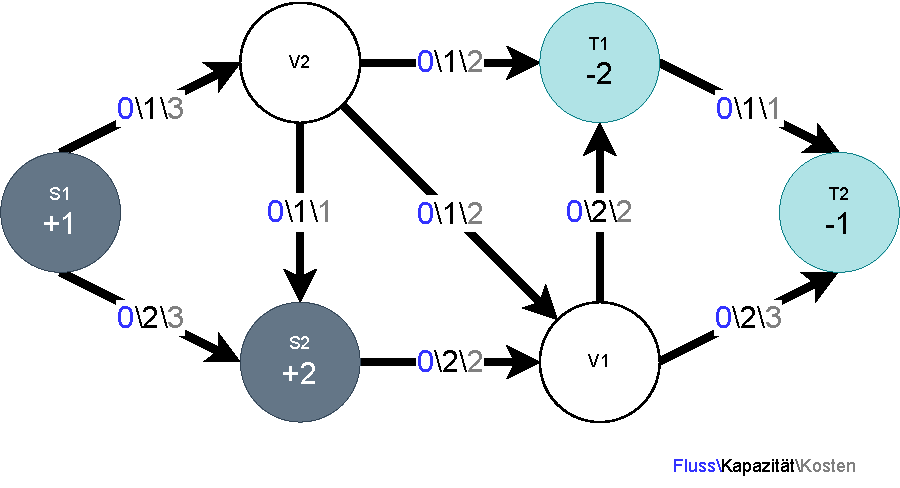
\includegraphics[width=0.8\textwidth]{img/anton/sspa-initial.pdf}
\caption{SSPA Initial}
\label{fig:sspa_initial}
\end{figure}

\begin{figure}[H]
\centering
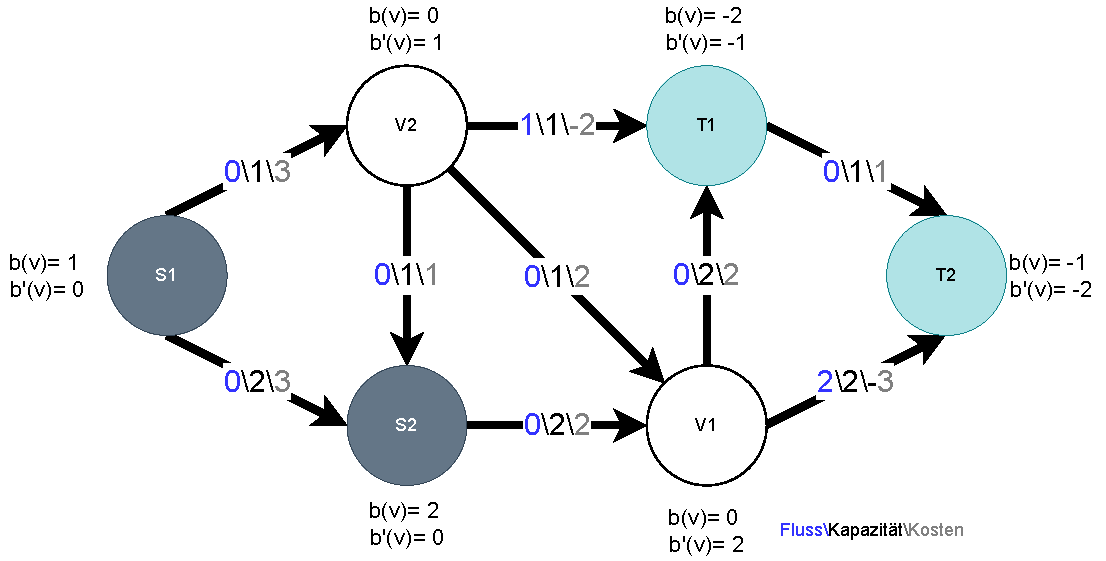
\includegraphics[width=0.9\textwidth]{img/anton/sspa-Step1.pdf}
\caption{SSPA Graph nach Schritt 1}
\label{fig:sspa_step1}
\end{figure}

In Abbildung \ref{fig:sspa_step1} ist der Graph nach Anwendung des ersten Schritts zu sehen. Die negativen Kanten sind maximiert, die restlichen Kanten auf $0$ gesetzt und jeder Knoten hat zu seiner Ziel-Balance $b(v)$ noch eine aktuelle Balance $b'(v)$ erhalten. Danach beginnt die erste Iteration.

\begin{figure}[H]
\centering
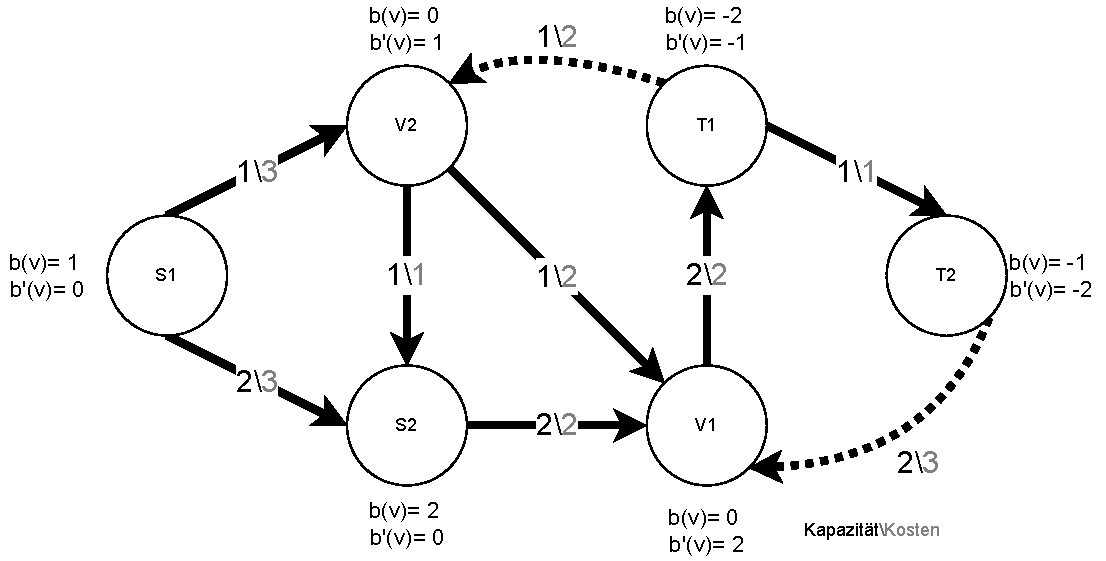
\includegraphics[width=0.9\textwidth]{img/anton/sspa-Step1-residual.pdf}
\caption{SSPA Iteration 1 Residualgraph}
\label{fig:sspa_step1-residual}
\end{figure}
%Reihenfolge noch anpassen?
Da es noch Quellen und Senken gibt, kann nun der Residualgraph aufgestellt werden um einen kürzesten Weg zwischen diesen zu finden. Dieser ist in Abbildung \ref{fig:sspa_step1-residual} zu sehen.

\begin{figure}[H]
\centering
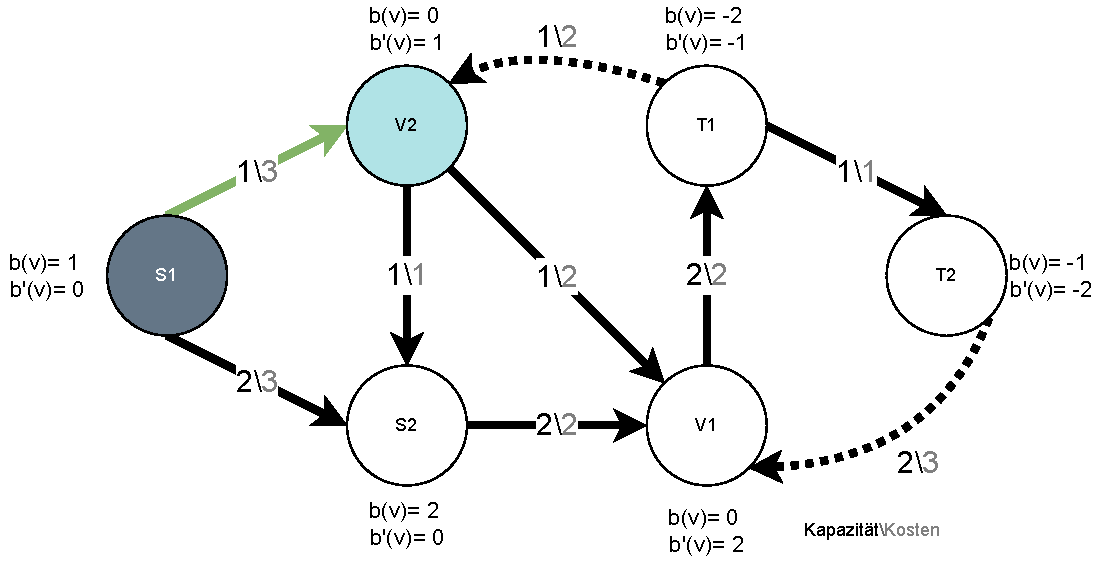
\includegraphics[width=0.9\textwidth]{img/anton/sspa-Step1-shortestPath.pdf}
\caption{SSPA Weg von $S1$ zu $V2$}
\label{fig:sspa_step1-shortestPath}
\end{figure}

In dem Beispiel wurde der Knoten $S1$ als Quelle und $V2$ als Senke verwendet (vgl. Abbildung \ref{fig:sspa_step1-shortestPath}. Nun kann mithilfe bspw. des Moore-Bellman-Ford-Algorithmus' ein kürzester Weg zueinander berechnet werden. Das Ergebnis davon ist hier grün eingezeichnet. Da ein kürzester Weg gefunden wurde, findet anschließend die Veränderung des Weges entlang des Flusses statt. Die Veränderung berechnet sich aus $\gamma := min\{\underset{e \in p}{min} \{u^f (e) \}, b(s) - b'(s), b'(t) - b(t)\} $, also $\gamma := min\{1, 1, 1\}$. In diesem Fall beträgt jeder der drei Werte $1$. An der Quelle und im Fluss finden daher eine Veränderung um $+1$ statt, während die Senke $-1$ erhält. Damit ist die erste Iteration beendet.

\begin{figure}[H]
\centering
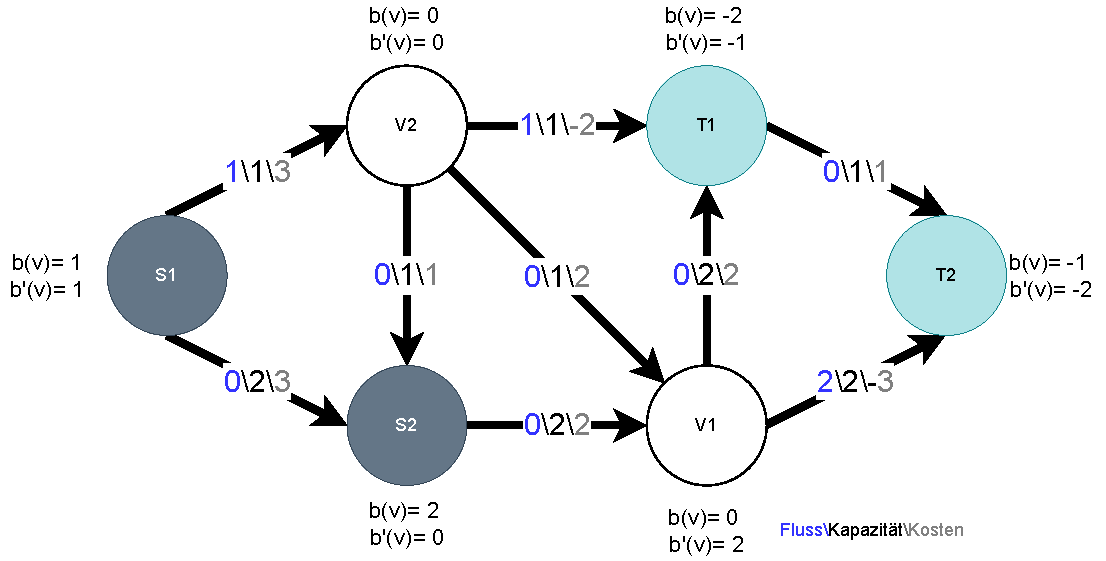
\includegraphics[width=0.9\textwidth]{img/anton/sspa-Step1-newGraph.pdf}
\caption{SSPA Graph nach Iteration 1}
\label{fig:sspa_step1-new-Graph}
\end{figure}

In Abbildung \ref{fig:sspa_step1-new-Graph} ist nun der Graph nach der ersten Iteration zu sehen. Anschließend beginnt die zweite Iteration.

\begin{figure}[H]
\centering
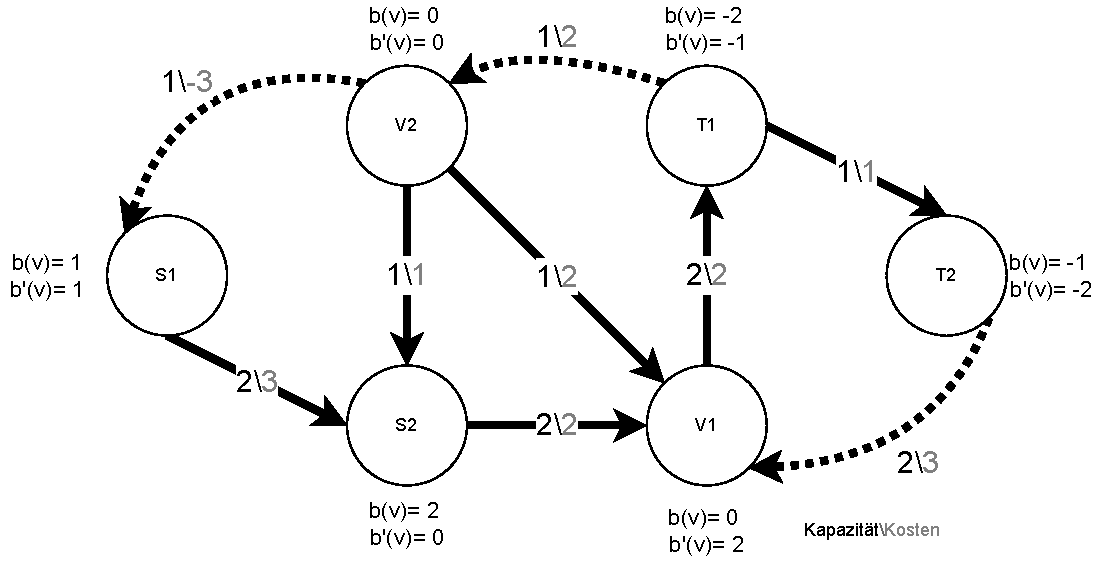
\includegraphics[width=0.9\textwidth]{img/anton/sspa-Step2-residual.pdf}
\caption{SSPA Iteration 2 Residualgraph}
\label{fig:sspa_step2-residual}
\end{figure}

Da es immer noch Quellen und Senken gibt, wird zu Beginn der zweiten Iteration erneut der Residualgraph gebildet (vgl. Abbildung \ref{fig:sspa_step2-residual}).

\begin{figure}[H]
\centering
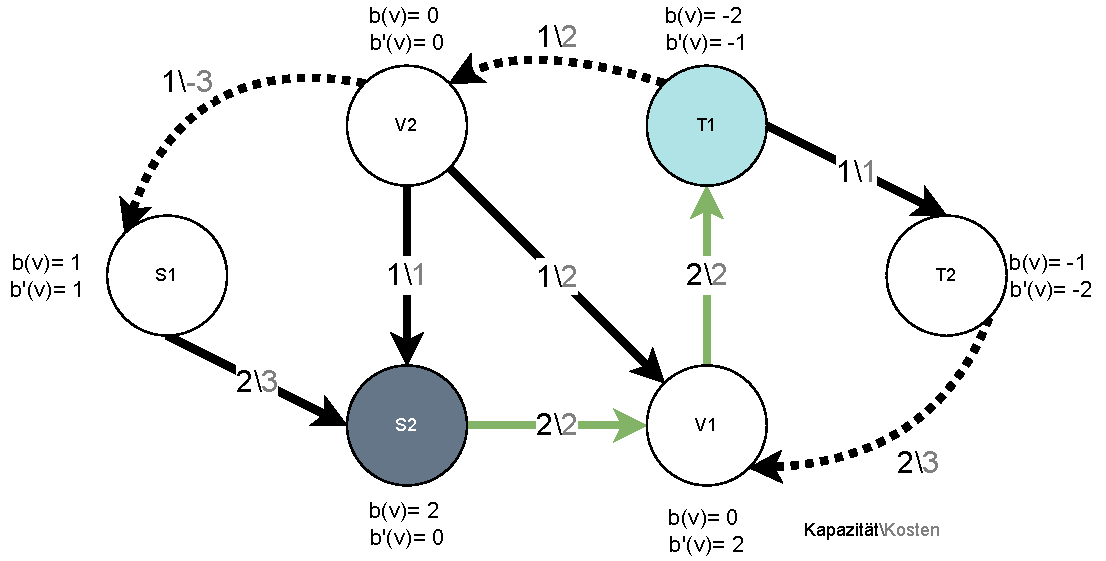
\includegraphics[width=0.9\textwidth]{img/anton/sspa-Step2-shortestPath.pdf}
\caption{SSPA Weg von $S2$ zu $T1$}
\label{fig:sspa_step2-shortestPath}
\end{figure}

\begin{figure}[H]
\centering
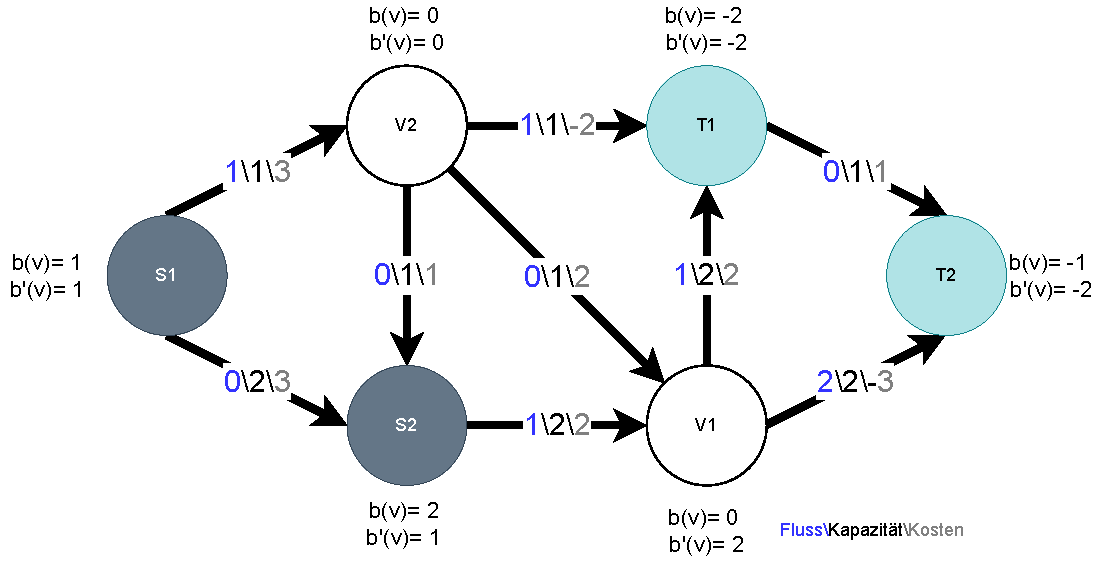
\includegraphics[width=0.9\textwidth]{img/anton/sspa-Step2-newGraph.pdf}
\caption{SSPA Graph nach Iteration 2}
\label{fig:sspa_step2-new-Graph}
\end{figure}

Anschließend wird erneut der kürzeste Weg zwischen Quelle und Senke gesucht (vgl. Abbildung \ref{fig:sspa_step2-shortestPath}). Das entstehende Gamma aus dem Weg von $S2$ zu $T1$ lautet $\gamma := min\{2, 2, 1\}$. Der Weg wird demnach erneut um den Wert $1$ verändert, wodurch der Graph aus Abbildung \ref{fig:sspa_step2-new-Graph} entsteht. Daraufhin startet die dritte Iteration mit dem Residualgraphen in Abbildung \ref{fig:sspa_step3-residual}.

\begin{figure}[H]
\centering
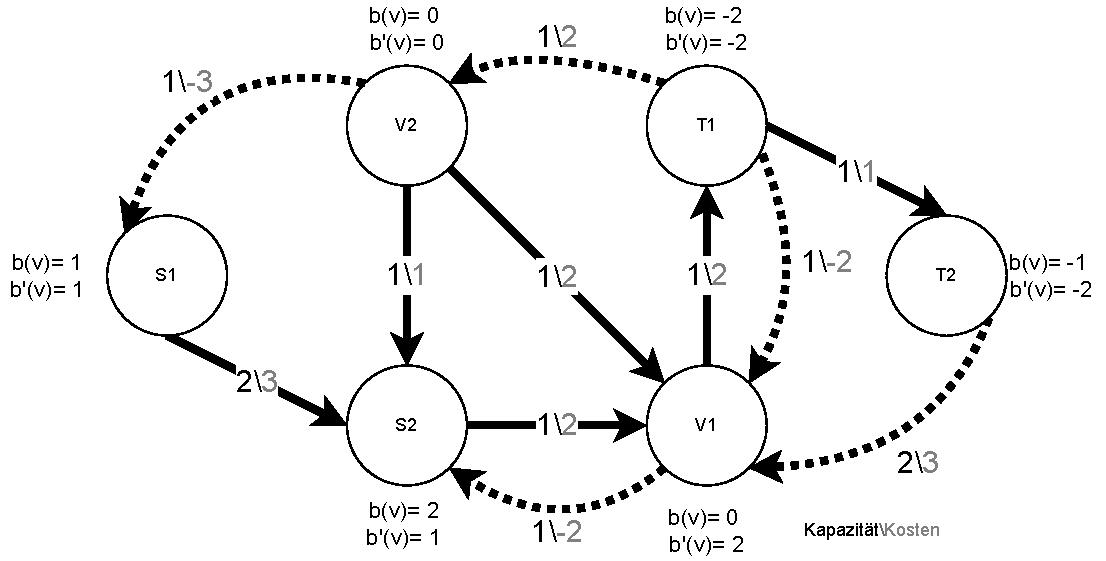
\includegraphics[width=0.9\textwidth]{img/anton/sspa-Step3-residual.pdf}
\caption{SSPA Iteration 3 Residualgraph}
\label{fig:sspa_step3-residual}
\end{figure}

\begin{figure}[H]
\centering
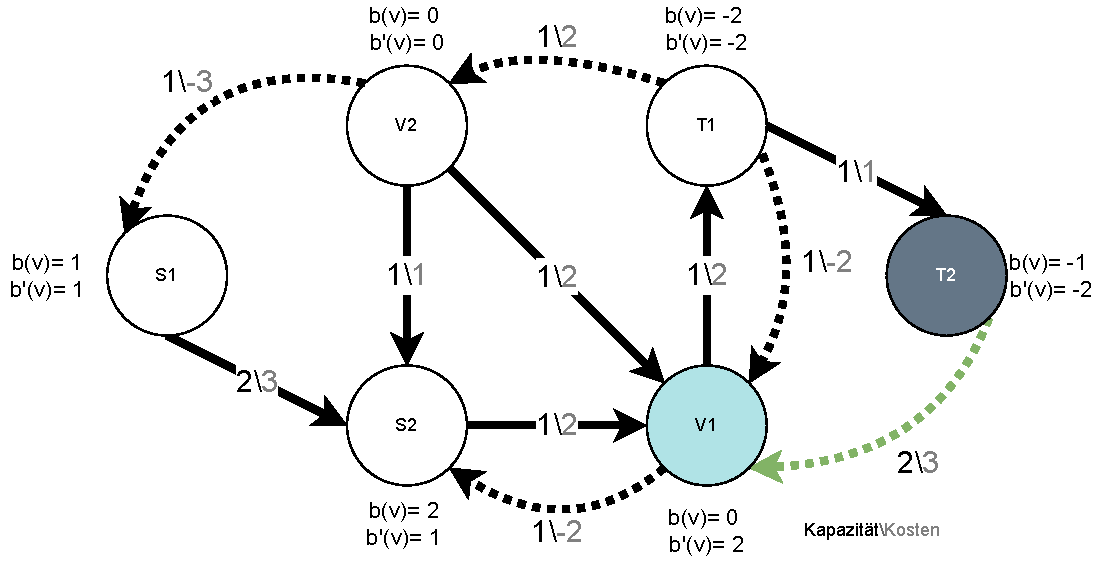
\includegraphics[width=0.9\textwidth]{img/anton/sspa-Step3-shortestPath.pdf}
\caption{SSPA Weg von $T2$ zu $V1$}
\label{fig:sspa_step3-shortestPath}
\end{figure}

In dem Graphen befinden sich noch zwei Quellen mit $S2$ und $T2$ und eine Senke mit $V1$. Es wird der Weg von $T2$ zu $V1$ mit dem entsprechenden kürzesten Weg gesucht (vgl. Abbildung \ref{fig:sspa_step3-shortestPath}. Das entstehende Gamma lautet: $\gamma := min\{2, 2, 1\}$, also 1. Nach der Veränderung entlang des Weges entsteht der Graph aus Abbildung \ref{fig:sspa_step3-new-Graph}.

\begin{figure}[H]
\centering
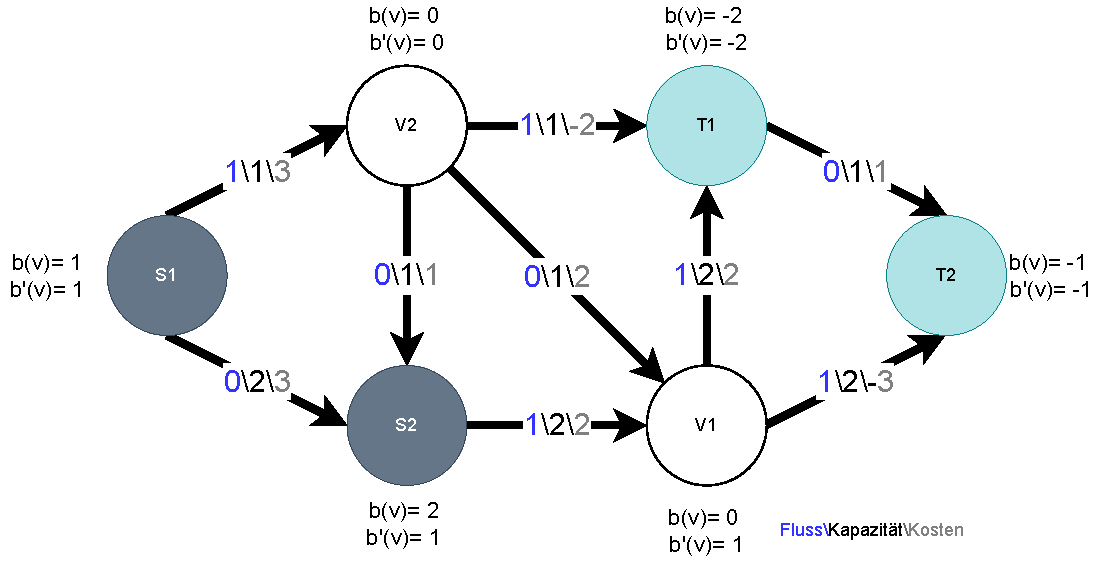
\includegraphics[width=0.9\textwidth]{img/anton/sspa-Step3-newGraph.pdf}
\caption{SSPA Graph nach Iteration 3}
\label{fig:sspa_step3-new-Graph}
\end{figure}

Aus dem Graphen geht es in die vierte Iteration mit dem Residualgraphen in Abbildung \ref{fig:sspa_step4-residual} und den verbleibenden Knoten $S2$ und $V1$, zwischen denen auch ein kürzester Weg mit $\gamma := min\{1, 1, 1\}$ gefunden werden kann (vgl. Abbildung \ref{fig:sspa_step4-shortest-Path}. Nachdem die Veränderung entlang des Weges abgeschlossen ist, entsteht der Graph aus Abbildung \ref{fig:sspa_step4-new-Graph}.

\begin{figure}[H]
\centering
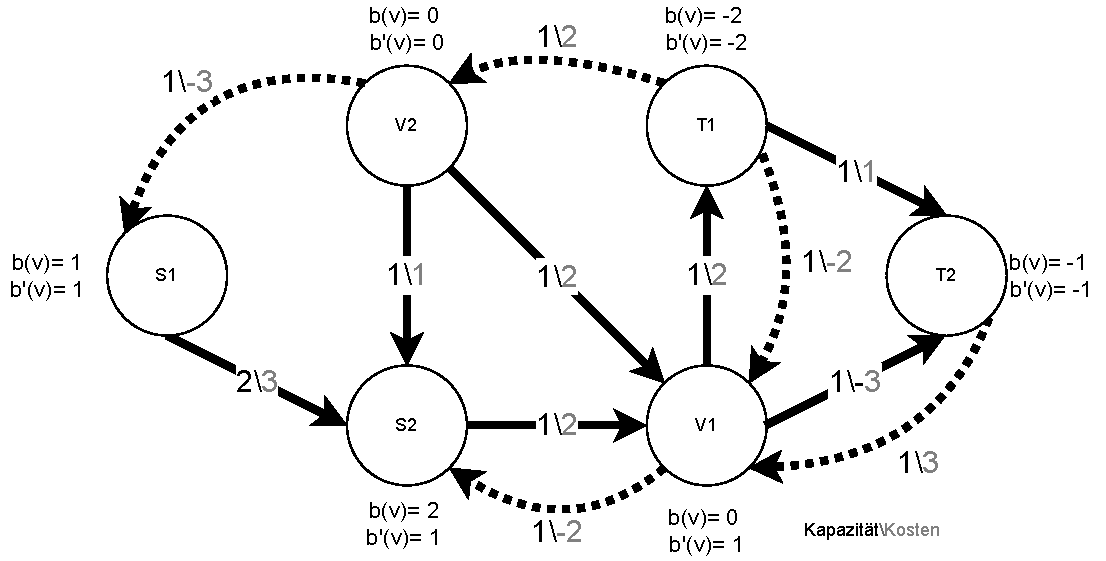
\includegraphics[width=0.9\textwidth]{img/anton/sspa-Step4-residual.pdf}
\caption{SSPA Iteration 4 Residualgraph}
\label{fig:sspa_step4-residual}
\end{figure}

\begin{figure}[H]
\centering
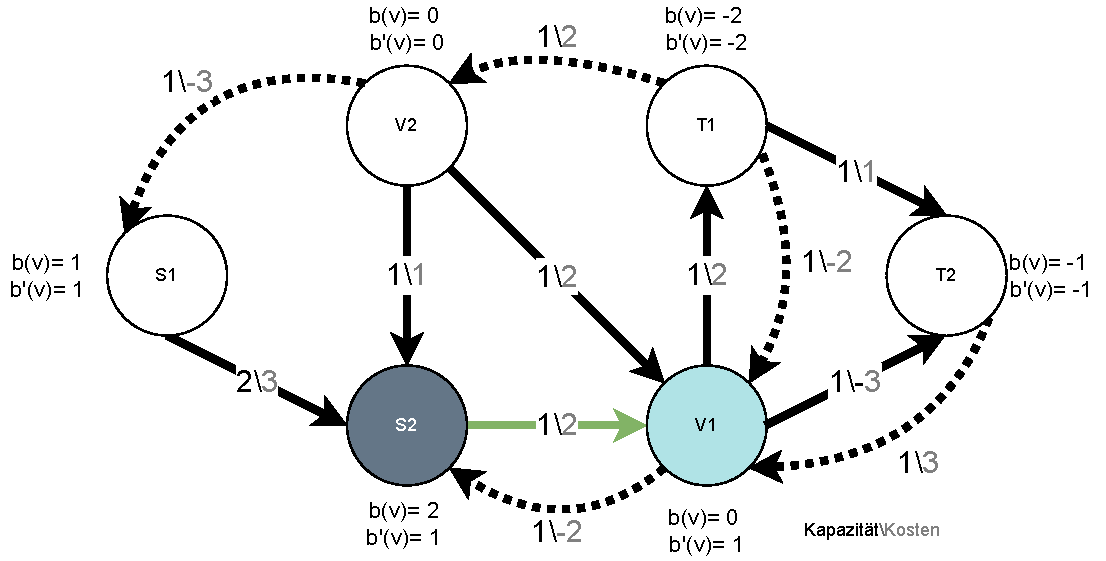
\includegraphics[width=0.9\textwidth]{img/anton/sspa-Step4-shortestPath.pdf}
\caption{SSPA Weg von $S2$ nach $V1$}
\label{fig:sspa_step4-shortest-Path}
\end{figure}

\begin{figure}[H]
\centering
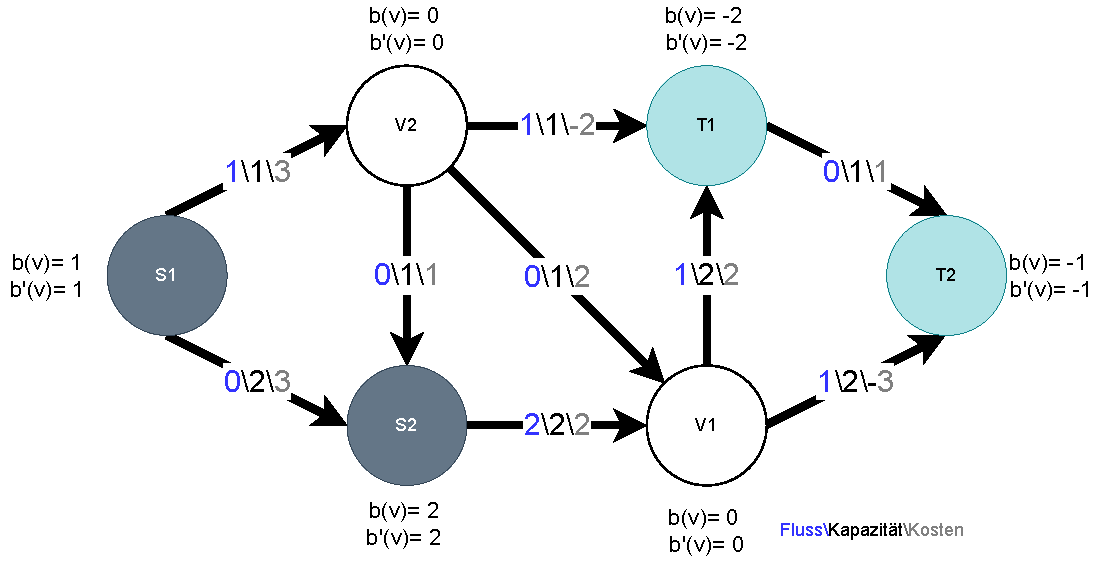
\includegraphics[width=0.9\textwidth]{img/anton/sspa-Step4-newGraph.pdf}
\caption{SSPA Graph nach Iteration 4}
\label{fig:sspa_step4-new-Graph}
\end{figure}

Da es keine Quellen und keine Senken mehr gibt, muss nun geprüft werden ob für alle Knoten $b(v) = b'(v)$ gilt. Da dies der Fall ist, findet sich der finale Graph mit den entstandenen Flusswerten in Abbildung \ref{fig:sspa_step5-final}.

\begin{figure}[H]
\centering
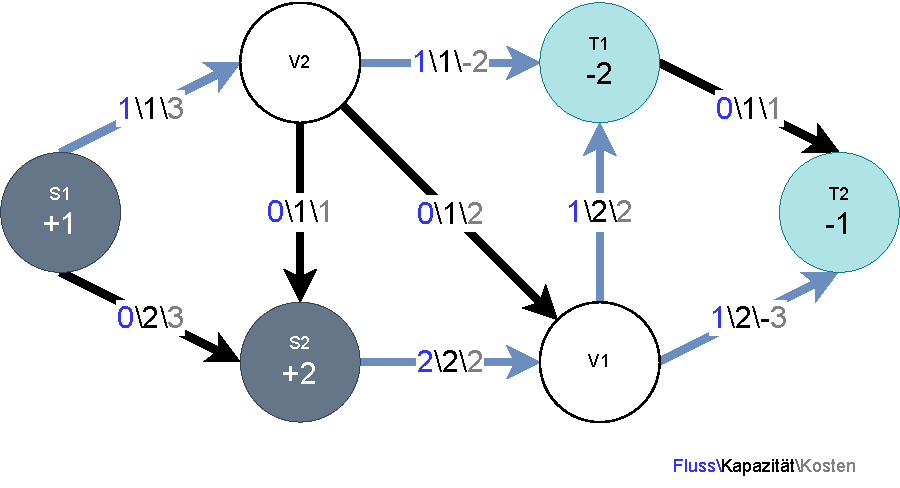
\includegraphics[width=0.8\textwidth]{img/anton/sspa-Step5-FinalMitFluss.pdf}
\caption{SSPA finaler Graph mit kostenminimalem $b$-Fluss}
\label{fig:sspa_step5-final}
\end{figure}

Um den finalen Wert zu errechnen muss nun die Formel aus Definition \ref{def:costfunktion} angewendet werden. Nach der Betrachtung aller Kanten ergeben sich die finalen Kosten von $4$.

\section{Fazit}
Der SSPA ist ein Weg um immer einen Kostenminimalen Fluss zu finden sofern er existiert. Des Weiteren darf im Verlauf des Algorithmus kein negativer Zykel auftreten, da dann der Moore-Bellmann-Ford-Algorithmus nicht mehr funktionieren würde. Zudem muss bei der Verwendung von ungerichteten Graphen darauf geachtet werden wie die Kanten aufgestellt werden. Weitere Informationen dazu finden sich bei \cite{sspa}. Die Komplexität des Algorithmus beträgt laut \cite{sspa} $O(n^2m^2)$ wobei es sich aus $O(nm) * T(n,m)$ zusammensetzt. Hierbei stellt T den Moore-Bellman-Ford-Algorithmus dar.

%%%%%%%%%%%%%%%%%%%%%%%%%%%%%%%%%%%%%%%%%%%%%%%%%%%%%%%%%%%%
% Verzeichnisse hinten
%%%%%%%%%%%%%%%%%%%%%%%%%%%%%%%%%%%%%%%%%%%%%%%%%%%%%%%%%%%%

\listoffigures
\addcontentsline{toc}{chapter}{\listfigurename}

\begingroup
    \let\clearpage\relax
    \listoftables
\endgroup
\addcontentsline{toc}{chapter}{\listtablename}


%%%%%%%%%%%%%%%%%%%%%%%%%%%%%%%%%%%%%%%%%%%%%%%%%%%%%%%%%%%%
% Literaturverzeichnis
%%%%%%%%%%%%%%%%%%%%%%%%%%%%%%%%%%%%%%%%%%%%%%%%%%%%%%%%%%%%


%% Verschiedene Versionen, nach DIN 1505 zu zitieren
%\bibliographystyle{plaindin}
%\bibliographystyle{natdin}
%\bibliographystyle{alphadin}
%\bibliographystyle{unsrtdin}

% Die DIN 1505 Styles müssen ggf. nachinstalliert werden. Bei Texlive
% heisst das Paket texlive-bibtex-extra

%Where the bibliography will be printed
\setlength{\parskip}{2pt}
\renewcommand{\bibname}{Quellenverzeichnis} % Umbenennung des Literaturverzeichnisses
\footnotesize
\bibliography{literatur}
%\printbibliography % Biblatex
\addcontentsline{toc}{chapter}{Quellenverzeichnis} % Eintrag ins Inhaltsverzeichnis

%%%%%%%%%%%%%%%%%%%%%%%%%%%%%%%%%%%%%%%%%%%%%%%%%%%%%%%%%%%%
% Anhang
%%%%%%%%%%%%%%%%%%%%%%%%%%%%%%%%%%%%%%%%%%%%%%%%%%%%%%%%%%%%

\clearpage
\appendix

%\chapter{Anhänge}

%\newcommand\includeappendixpdf[2]{}

%\include{anhang/Umfrage-Datentabelle}

%\includepdf{anhang/BeliebigesDokument.pdf}{Test}

%\chapter{Sonstiges}

\end{document}